\documentclass[a4paper,11pt]{book}
%\documentclass[a4paper,twoside,11pt,titlepage]{book}
\usepackage{indentfirst}
\usepackage{listings}
\usepackage{booktabs,siunitx}
\usepackage[utf8]{inputenc}
\usepackage[spanish]{babel}
\usepackage{amsmath}
\usepackage{xcolor}
\usepackage{tcolorbox}
\usepackage{amsmath}
\usepackage{array}
\usepackage{tabulary}
\usepackage{multirow}
\tcbuselibrary{breakable}
\usepackage{lipsum}
% \usepackage[style=list, number=none]{glossary} %
%\usepackage{titlesec}
%\usepackage{pailatino}

\decimalpoint
\usepackage{dcolumn}
\newcolumntype{.}{D{.}{\esperiod}{-1}}
\makeatletter
\addto\shorthandsspanish{\let\esperiod\es@period@code}
\makeatother


%\usepackage[chapter]{algorithm}
\RequirePackage{verbatim}
%\RequirePackage[Glenn]{fncychap}
\usepackage{fancyhdr}
\usepackage{graphicx}
\usepackage{afterpage}

\usepackage{longtable}

\usepackage[pdfborder={000}]{hyperref} %referencia

% ********************************************************************
% Re-usable information
% ********************************************************************
\newcommand{\myTitle}{Cryptanalysis Ciphertext Based Genetic Algorithms\xspace}
\newcommand{\myDegree}{Master Universitario en INGENIERÍA INFORMÁTICA\xspace}
\newcommand{\myName}{Abdullah Taher Saadoon AL Muswai (alumno)\xspace}
\newcommand{\myProf}{Juan Julián Merelo Guervós (tutor)\xspace}

%\newcommand{\mySupervisor}{Put name here\xspace}
\newcommand{\myFaculty}{Escuela Técnica Superior de Ingenierías Informática y de
Telecomunicación\xspace}
\newcommand{\myFacultyShort}{E.T.S. de Ingenierías Informática y de
Telecomunicación\xspace}

\newcommand{\myUni}{\protect{Universidad de Granada}\xspace}
\newcommand{\myLocation}{Granada\xspace}
\newcommand{\myTime}{\today\xspace}
\newcommand{\myVersion}{Version 0.1\xspace}


\hypersetup{
pdfauthor = {\myName abdullahtaher@correo.ugr.es},
pdftitle = {\myTitle},
pdfsubject = {},
pdfkeywords = {palabra_clave1, palabra_clave2, palabra_clave3, ...},
pdfcreator = {LaTeX con el paquete ....},
pdfproducer = {pdflatex}
}

%\hyphenation{}


%\usepackage{doxygen/doxygen}
%\usepackage{pdfpages}
\usepackage{url}
\usepackage{colortbl,longtable}
\usepackage[stable]{footmisc}
%\usepackage{index}

%\makeindex
%\usepackage[style=long, cols=2,border=plain,toc=true,number=none]{glossary}
% \makeglossary

% Definición de comandos que me son tiles:
%\renewcommand{\indexname}{Índice alfabético}
%\renewcommand{\glossaryname}{Glosario}

\pagestyle{fancy}
\fancyhf{}
\fancyhead[LO]{\leftmark}
\fancyhead[RE]{\rightmark}
\fancyhead[RO,LE]{\textbf{\thepage}}
\renewcommand{\chaptermark}[1]{\markboth{\textbf{#1}}{}}
\renewcommand{\sectionmark}[1]{\markright{\textbf{\thesection. #1}}}

\setlength{\headheight}{1.5\headheight}

\newcommand{\HRule}{\rule{\linewidth}{0.5mm}}
%Definimos los tipos teorema, ejemplo y definición podremos usar estos tipos
%simplemente poniendo \begin{teorema} \end{teorema} ...
\newtheorem{teorema}{Teorema}[chapter]
\newtheorem{ejemplo}{Ejemplo}[chapter]
\newtheorem{definicion}{Definición}[chapter]

\definecolor{gray97}{gray}{.97}
\definecolor{gray75}{gray}{.75}
\definecolor{gray45}{gray}{.45}
\definecolor{gray30}{gray}{.94}

\lstset{ frame=Ltb,
     framerule=0.5pt,
     aboveskip=0.5cm,
     framextopmargin=3pt,
     framexbottommargin=3pt,
     framexleftmargin=0.1cm,
     framesep=0pt,
     rulesep=.4pt,
     backgroundcolor=\color{gray97},
     rulesepcolor=\color{black},
     %
     stringstyle=\ttfamily,
     showstringspaces = false,
     basicstyle=\scriptsize\ttfamily,
     commentstyle=\color{gray45},
     keywordstyle=\bfseries,
     %
     numbers=left,
     numbersep=6pt,
     numberstyle=\tiny,
     numberfirstline = false,
     breaklines=true,
   }

% minimizar fragmentado de listados
\lstnewenvironment{listing}[1][]
   {\lstset{#1}\pagebreak[0]}{\pagebreak[0]}

\lstdefinestyle{CodigoC}
   {
	basicstyle=\scriptsize,
	frame=single,
	language=C,
	numbers=left
   }
\lstdefinestyle{CodigoC++}
   {
	basicstyle=\small,
	frame=single,
	backgroundcolor=\color{gray30},
	language=C++,
	numbers=left
   }


\lstdefinestyle{Consola}
   {basicstyle=\scriptsize\bf\ttfamily,
    backgroundcolor=\color{gray30},
    frame=single,
    numbers=none
   }


\newcommand{\bigrule}{\titlerule[0.5mm]}


%Para conseguir que en las páginas en blanco no ponga cabecerass
\makeatletter
\def\clearpage{%
  \ifvmode
    \ifnum \@dbltopnum =\m@ne
      \ifdim \pagetotal <\topskip
        \hbox{}
      \fi
    \fi
  \fi
  \newpage
  \thispagestyle{empty}
  \write\m@ne{}
  \vbox{}
  \penalty -\@Mi
}
\makeatother

\usepackage{pdfpages}

\begin{document}
\begin{titlepage}


\newlength{\centeroffset}
\setlength{\centeroffset}{-0.5\oddsidemargin}
\addtolength{\centeroffset}{0.5\evensidemargin}
\thispagestyle{empty}

\noindent\hspace*{\centeroffset}\begin{minipage}{\textwidth}

\centering

\includegraphics[width=0.9\textwidth]{imagenes/logo_ugr.jpg}\\[1.4cm]

\textsc{ \Large TRABAJO FIN DE MASTER\\[0.2cm]}
\textsc{ INGENIERÍA INFORMÁTICA}\\[1cm]
% Upper part of the page
%
% Title
{\LARGE\bfseries Cryptanalysis Ciphertext Based Genetic Algorithms\\
}
\noindent\rule[-1ex]{\textwidth}{3pt}\\[3.5ex]
{\large\bfseries Breaking Transposition and Substitution Ciphers with Genetic Algorithm}
\end{minipage}

\noindent\hspace*{\centeroffset}\begin{minipage}{\textwidth}
\centering
\vspace{0.6cm}
\textbf{Autor}\\ {Abdullah Taher Saadoon AL Muswai (alumno)}\\[2.5ex]
\textbf{Directores}\\{Juan Julián Merelo Guervós (tutor)}\\[2cm]

\includegraphics[width=0.3\textwidth]{imagenes/etsiit_logo.png}\\[0.1cm]
\textsc{Escuela Técnica Superior de Ingenierías Informática y de Telecomunicación}\\
\textsc{---}\\
Granada, septiembre de 2020
\end{minipage}
%\addtolength{\textwidth}{\centeroffset}
%\vspace{\stretch{2}}
\end{titlepage}



\chapter*{}
%\thispagestyle{empty}
%\cleardoublepage

%\thispagestyle{empty}

\begin{titlepage}
 
 
\setlength{\centeroffset}{-0.5\oddsidemargin}
\addtolength{\centeroffset}{0.5\evensidemargin}
\thispagestyle{empty}

\noindent\hspace*{\centeroffset}\begin{minipage}{\textwidth}

\centering
%
\includegraphics[width=0.9\textwidth]{imagenes/logo_ugr.jpg}\\[1.4cm]

%\textsc{ \Large PROYECTO FIN DE CARRERA\\[0.2cm]}
%\textsc{ INGENIERÍA EN INFORMÁTICA}\\[1cm]
% Upper part of the page
% 

 \vspace{3.3cm}

%si el proyecto tiene logo poner aquí

 \vspace{0.5cm}

% Title

{\Huge\bfseries Cryptanalysis Ciphertext Based Genetic Algorithms\\
}
\noindent\rule[-1ex]{\textwidth}{3pt}\\[3.5ex]
{\large\bfseries  Breaking Transposition and Substitution Ciphers with Genetic Algorithm.\\[4cm]}
\end{minipage}

\vspace{2.5cm}
\noindent\hspace*{\centeroffset}\begin{minipage}{\textwidth}
\centering

\textbf{Autor}\\ {Abdullah Taher Saadoon AL Muswai (alumno)}\\[2.5ex]
\textbf{Directores}\\{Juan Julián Merelo Guervós (tutor)}\\[2cm]
%\includegraphics[width=0.15\textwidth]{imagenes/tstc.png}\\[0.1cm]
%\textsc{Departamento de Teoría de la Señal, Telemática y Comunicaciones}\\
%\textsc{---}\\
%Granada, mes de 201
\end{minipage}
%\addtolength{\textwidth}{\centeroffset}
\vspace{\stretch{2}}

 
\end{titlepage}






\cleardoublepage

\thispagestyle{empty}


\begin{center}
{\large\bfseries Cryptanalysis Ciphertext Based Genetic Algorithms: Breaking Transposition and Substitution Ciphers with Genetic Algorithm}\\
\end{center}
\begin{center}
Abdullah, AL Musawi(student)\\
\end{center}

%\vspace{0.7cm}
\noindent{\textbf{Keywords}: Cryptanalysis, Genetic Algorithm, Transposition Cipher, substitution
cipher, decryption ,optimization search.}\\

\vspace{0.7cm}
\noindent{\textbf{Abstract}}\\

This thesis describes a method of deciphering messages encrypted with transposition cipher and substitution cipher utilising a Genetic Algorithm to search the keyspace.
There are many tools used in the cryptanalysis, Genetic algorithm(GA) is an optimization search tool to find the best solution.

In this project, A fitness measure based on \textbf{English Letter Frequencies} for random of text is described which got it by generating random popultaion. 
The results are compared to those given using a previously published technique and found to be superior.

\chapter*{}
\thispagestyle{empty}

\noindent\rule[-1ex]{\textwidth}{2pt}\\[4.5ex]

Yo, \textbf{Abdullah Taher Saadoon AL Muswai}, alumno de la titulación  máster de Ingeniería Informática  de la \textbf{Escuela Técnica Superior de Ingenierías Informática y de Telecomunicación de la Universidad de Granada}, con DNI A11518169, autorizo la
ubicación de la siguiente copia de mi Trabajo Fin de Master en la biblioteca del centro para que pueda ser
consultada por las personas que lo deseen.

\vspace{6cm}

\noindent Fdo: Abdullah Taher Saadoon AL Muswai

\vspace{2cm}

\begin{flushright}
Granada a 10 de septimpre de 2020.
\end{flushright}


\chapter*{}
\thispagestyle{empty}

\noindent\rule[-1ex]{\textwidth}{2pt}\\[4.5ex]

D. \textbf{ Juan Julián Merelo Guervos (tutor)}, Profesor del Departamento de Arquitectura y Tecnología de Computadores de la Universidad de Granada.

\vspace{0.5cm}



\vspace{0.5cm}

\textbf{Informan:}

\vspace{0.5cm}

Que el presente trabajo, titulado \textit{\textbf{Cryptanalysis Ciphertext Based Genetic Algorithms,Breaking Transposition and Substitution Ciphers with Genetic Algorithm}},
ha sido realizado bajo su supervisión por \textbf{Abdullah Taher Saadoon AL Muswai (alumno)}, y autorizamos la defensa de dicho trabajo ante el tribunal
que corresponda.

\vspace{0.5cm}

Y para que conste, expiden y firman el presente informe en Granada a X de mes de 201 .

\vspace{1cm}

\textbf{Los directores:}

\vspace{5cm}

\noindent \textbf{Juan Julián Merelo Guervos (tutor) \ \ }

\chapter*{Agradecimientos}
\thispagestyle{empty}

       \vspace{1cm}


Poner aquí agradecimientos...


\frontmatter
\tableofcontents
\listoffigures
\listoftables

\mainmatter
\setlength{\parskip}{5pt}

\chapter{Introduction}

Cryptanalysis is the technique of deriving the original message from the cipher text without any prior knowledge of secret key or the erivation of key from the cipher text. A general technique for cryptanalysis, applied to all cryptographic algos is to try all the possible keys until the correct key is matched, it is known as exhaustive key search. 

With every passing day, the computing ability of hardware is increasing manifold; therefore it becomes necessary to use long keys for avoiding exhaustive key search. All the other attacks applied to stream ciphers are compared to exhaustive key search in terms of data and memory complexity and if its complexity is less than exhaustive key search, then only these are considered as successful. 

A symmetric key cipher, especially a stream cipher is assumed secure, if the computational capability required for breaking the cipher by
best-known attack is greater than or equal to exhaustive key search. 
Cryptanalysis is the science of making encrypted data unencrypted use convert cipher text to plaintext because cryptanalysis used to convert
plaintext to cipher text and used cryptanalysis Return to plaintext or clear text or original text cryptanalysis is used to break codes by finding
weaknesses. There are many techniques used in the cryptanalysis. This project used the genetics algorithm \cite{bokhari2012cryptanalysis}.

The genetic algorithm is a search algorithm based on the mechanics of natural selection and natural genetics. The genetic algorithm belongs to
 the family of evolutionary algorithms, along with genetic programming,
Evolution strategies and evolutionary programming. The set of operators
usually consists of mutation, crossover and selection \cite{mangano1995genetic}.

\newpage
A genetic
algorithm has proven to be reliable and powerful optimization technique in
a wide variety of applications. It can be applied to both texts and images.
Genetic algorithm is secure since it does not utilize the natural numbers
directly. The genetic algorithm used for generating keys that it should be
good in terms of coefficient of autocorrelation \cite{sindhuja2014symmetric}.

Apply the technique of
genetic algorithms to the problem of finding the key to a particular
Transposition Cipher. Since Genetic Algorithms are primarily used to
efficiently search a large problem space we thought they would be ideally
suited for searching the large key space \cite{brownbridge2007decrypting}.

\section{aim of the project}
The main purpose of the project is examine the possible applications of genetic
algorithms in cryptology,with the emphasis of the research being in the application of a genetic algorithm in the  which explores the
plaintext from cipher text based on genetic algorithm (GA) which is used
for suggesting decryption key. The genetic algorithm (GA) is a search tool
to insure high probability of finding a solution by decreasing the amount
of time in the key space searching.
this project covers two ciphers type: Transposition Cipher and Substitution Cipher. 
We present a review of Transposition Cipher ,Substitution Cipher, English Letter Frequencies and genetic algorithm in chapters ***** which provides
enough background to understand the techniques applied and to assess the
usefulness of the results obtained.
\section{project organization}
In additional to chapter one (the introduction), this project is
organized into three other chapters:
-Chapter * \textbf{" Theoretical Background"} this chapter introduces terms,
definitions, and descriptions that are used frequently throughout this
chapter. These terms focus on Cryptanalysis, Transposition Cipher, and
description Genetic algorithm (GA).
Chapter Three \textbf{" Design and Implementation: Cryptanalysis based on
Genetic Algorithm"} this chapter shows the design of the project and
explains the algorithms that support this work.
Chapter Four \textbf{"Conclusions and Future Work"} this chapter concludes
this project and finding the outline future works in the area of
Cryptanalysis.
\newpage
\chapter{Planning}

This chapter presents the work plan to follow to carry out this study. First of all, the requirements necessary to achieve the proposed objective will be captured, and then the work planning will be detailed, with an estimate of both work and material costs as well as a distribution of time between tasks.

\section{Investigation stages}
The steps of the research process of this study are as follows:

\begin{enumerate}
    \item{\textbf{Initiate a preliminary investigation of the Cryptanalysis:} review many of theses and papers looking for information about Cryptanalysis, check what evolution they have followed over the years and how the Cryptanalysis systems have been developed.}
    \item{\textbf{delve into the Transposition and Substitution ciphers:} investigate further in these types that are really going to focus on the study}
    \item {\textbf{Select the algorithm:} investigated in the previous steps, deciding the most appropriate option.}
    \item {\textbf{delve into genetic algorithm:} Study and understand all stages of genetic algorithm evolution and how to solve current problems, review the papers that related with GA.}
    \item {\textbf{Implement genetic algorithm:} create a set of classes, each of them performs stage of GA stages and all of them has a set of methods to divide its stage to small tasks every task solves a different problem.}
    \item {\textbf{create a new proposal for the study:} for the objective of the study, new proposals that can compete with the state of the art must be proposed.}
    \item {\textbf{Implement my new proposal:} that will be part of the experiment have been decided, they must be implemented in the same way as the state of the art algorithm. Check of new that all the functionality of the experiment is valid with the new implementation.}
    \item {\textbf{Obtain the results of the experiment:} obtain through the implementation of the experiment, can visualize the data in tables and graphs that are suitable for the study.}
    \item {\textbf{analysis of the results obtained:} compare the results of each method with the \textit{baseline} reference method and with the state of the art method, as well as between them, to discover which method behaves best for each case.}
    \item {\textbf{Consider future work to be done:} assess the aspects it is possible to continue progressing in the methods proposed in the study, propose new tasks or challenges within this field of research, that have not been covered in this study.}
\end{enumerate}

\section{Work plan}
This section is subdivided into cost estimation and time estimation. In the first place, The cost of the infrastructure used is evaluated, as long as the material that has been used is available for free and free. From there we can make a base budget from which to start. The time estimate should be realistic and meet the requirements within a competent time frame so that you do not need to postpone times at the last minute due to poor planning. If so, it would be necessary to bear the consequent increase in costs.
\subsection{Cost estimate of materials and infrastructure}
First of all, the computer with which this study has been developed will be taken, the following hardware and software have been used for this study:
\textbf{Computer Type:}Lenovo IdeaPad Z510.
\textbf{Processor:}Intel(R) Core(TM) i7-4702MQ CPU@ 2.20GHz 2.20GHz.
\textbf{Installed memory (RAM):} 8.00 GB.
\textbf{graphics card:} Intel(R) HD Graphics 4600, Memory:2176 MB.
\textbf{Hard Disk:} HDD 1TB

\textbf{Operating system:} Win10.
\textbf{Programming language:} java.
\textbf{Environment:}  NetBeans 8.1.
All the research, implementation, and evaluation tasks have been carried out with this team: documentation, review of the literature, writing of the report, development, implementation of the algorithms, and execution of the experiment to obtain results.

information and documentation required for the work are available  at the University of Granada  Thanks to the agreements that the University establishes with some documentary databases such as Scopus, it has been possible to access a multitude of papers and theses on the subject to be investigated. Furthermore, the Google scholer has been very useful to access other papers not found in Scopus.

The development of the work has been carried out entirely on the Win10 OS, The main software tools used have been open source so they have not entailed additional cost, Netbeans as the main IDE for development and writing the report of the project in LaTeX using the TeXstudio, available for win 10, and  we used  Visual Studio Code as an IDE to deal with the repository of the project that has hosted on \textbf{GitHub} \cite{MyProject} platform, and we used \textbf{Travis CI} \cite{travis_CI} to host continuous integration service used to build and test software projects hosted at GitHub,Travis CI provides various paid plan for private projects, and a free plan for open source.
Of all this material exposed in the previous paragraphs, the work has only required buying the personal laptop and the broadband network available, The rest of the infrastructure and materials have either been free software products or have been contributed by the University of Granada.

\subsection{Time distribution to the tasks}
we used the concepts of iterations and sprints to distribute the work throughout the weeks, in which a series of tasks have been developed that they fulfill a specific objective.

The Iteration and Sprint Planning meeting is for team members to plan and agree on the stories or backlog items they are confident they can complete during the sprint and identify the detailed tasks and tests for delivery and acceptance

The planning that has been foreseen for the development of the project is as follows:

\begin{table}[h!]
    \centering
    \begin{tabular}{|p{5cm}|p{4cm}|}
     \hline
        \cellcolor[gray]{0.9} Weeks  & 10 \\ \hline
        \cellcolor[gray]{0.9} Estimated total time (h)  & 240h \\ \hline
        \cellcolor[gray]{0.9} date of Starting Point  & 01-06-2020 \\ \hline
        \cellcolor[gray]{0.9} date of end Point   & 10-09-2020 \\ \hline
            
    \end{tabular}
    \end{table}

\subsection{Preparatory phase}
In this phase, the development of the project will begin, which has an estimated effort of 40 hours. A feasibility study of the project idea will be carried out, an investigation about the possible tools to use


\large{\underline{\textbf{Iteration 1}: Analysis and study of the project.}}
\vspace{0.3cm}
\begin{table}[h!]
    \centering
    \begin{tabular}{|p{5cm}|p{4cm}|}
     \hline
        \cellcolor[gray]{0.9} week  & 1\\ \hline
        \cellcolor[gray]{0.9} Total expected time (h)  & 40h \\ \hline
        \cellcolor[gray]{0.9} date of Starting Point  & 01-06-2020 \\ \hline
        \cellcolor[gray]{0.9} date of end Point  & 06-06-2020 \\ \hline
            
\end{tabular}
\end{table}

\textbf{Sprint 1}: Description of the Project

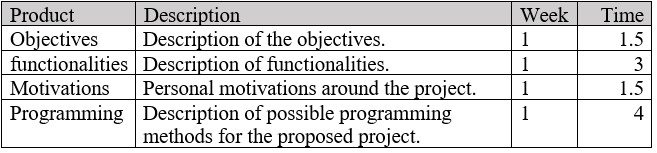
\includegraphics[width=0.9\textwidth]{imagenes/it1sp1.png}\\[1.4cm]
\textbf{Sprint 2}: Research and preparation of the environment.

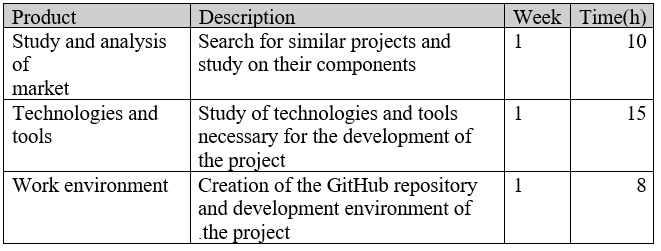
\includegraphics[width=0.9\textwidth]{imagenes/it1sp2.png}\\[1.4cm]

\subsection{Implementation and testing phase}

the objective of this phase is getting an general idea of this project and at the end of this phase, a software-implemented incrementally have been obtained, where each module has been tested until integration and validation.
A total of 280 hours has been planned for this phase, and it has been distributed in the following iterations:

\large{\underline{\textbf{Iteration 2}: Implementation of the main classes.}}
\vspace{0.3cm}

The objective of this iteration is the implementation of the main classes  which will create the system,For this operation, the following schedule has been established:

\begin{table}[h!]
    \centering
    \begin{tabular}{|p{5cm}|p{4cm}|}
     \hline
        \cellcolor[gray]{0.9} week  & 6\\ \hline
        \cellcolor[gray]{0.9} Total expected time (h)  & 120h \\ \hline
        \cellcolor[gray]{0.9} date of Starting Point  & 07-06-2020 \\ \hline
        \cellcolor[gray]{0.9} date of end Point  & 18-07-2020 \\ \hline
            
\end{tabular}
\end{table}

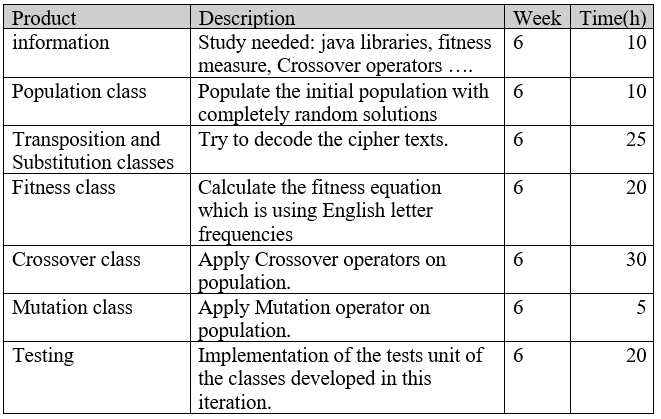
\includegraphics[width=0.9\textwidth]{imagenes/it2.png}\\[1.4cm]

\large{\underline{\textbf{Iteration 3}: Experimental results and Improvement.}}
\vspace{0.3cm}
The objective of this iteration is trying to get a result from the classes then try to improve all of them to get better results,For this iteration, the following schedule has been established:

\begin{table}[h!]
    \centering
    \begin{tabular}{|p{5cm}|p{4cm}|}
     \hline
        \cellcolor[gray]{0.9} week  & 10\\ \hline
        \cellcolor[gray]{0.9} Total expected time (h)  & 120h \\ \hline
        \cellcolor[gray]{0.9} date of Starting Point  & 18-07-2020 \\ \hline
        \cellcolor[gray]{0.9} date of end Point  & 18-08-2020 \\ \hline
            
\end{tabular}
\end{table}

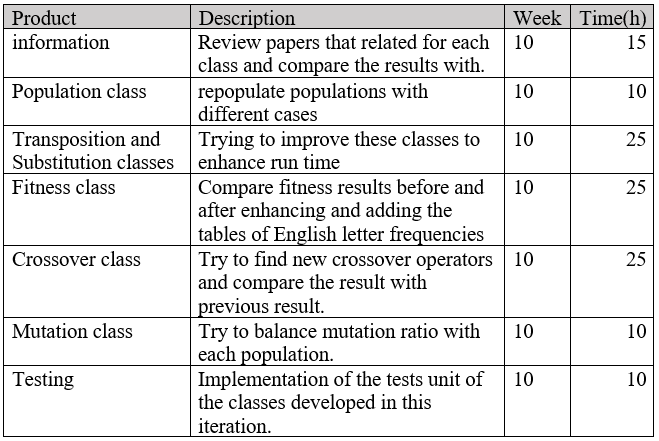
\includegraphics[width=0.9\textwidth]{imagenes/it3.png}\\[1.4cm]

\subsection{Documentation phase}
After the project is completed and approved, it is time to document all of the steps and how to work, and document the achieving result.

the documentations have been divided into two parts. The first one corresponds to the documentation in the Github repository. This documentation has as objective to give an idea about the project in general then delve in details until arrives in programming steps that explain all of the class and their methods and variables,  Anyone who accesses to the repository, he can see all this information as a free software project.

Other documents made are those for the project. In this case, more documentation focused on the scope of the project will be implemented: planning, research, development, Conclusions.
\newpage
\large{\underline{\textbf{Iteration 4}: GitHub Documentation.}}
In this phase has an estimated effort of 50 hours.

\begin{table}[h!]
    \centering
    \begin{tabular}{|p{5cm}|p{4cm}|}
     \hline
        \cellcolor[gray]{0.9} week  & 11\\ \hline
        \cellcolor[gray]{0.9} Total expected time (h)  & 50h \\ \hline
        \cellcolor[gray]{0.9} date of Starting Point  & 18-08-2020 \\ \hline
        \cellcolor[gray]{0.9} date of end Point  & 24-08-2020 \\ \hline
            
\end{tabular}
\end{table}

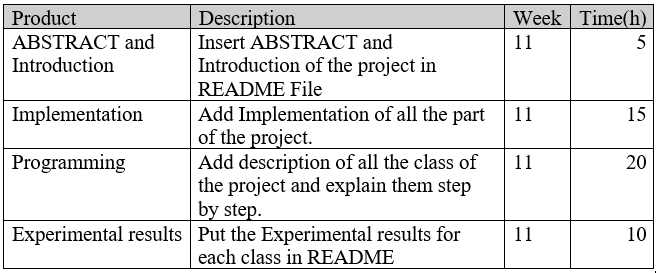
\includegraphics[width=0.9\textwidth]{imagenes/it4.png}\\[1.4cm]

\large{\underline{\textbf{Iteration 5}: Project documentation.}}

In this phase has an estimated effort of 150 hours.

\begin{table}[h!]
    \centering
    \begin{tabular}{|p{5cm}|p{4cm}|}
     \hline
        \cellcolor[gray]{0.9} week  & 13\\ \hline
        \cellcolor[gray]{0.9} Total expected time (h)  & 150h \\ \hline
        \cellcolor[gray]{0.9} date of Starting Point  & 24-08-2020 \\ \hline
        \cellcolor[gray]{0.9} date of end Point  & 09-09-2020 \\ \hline
            
\end{tabular}
\end{table}

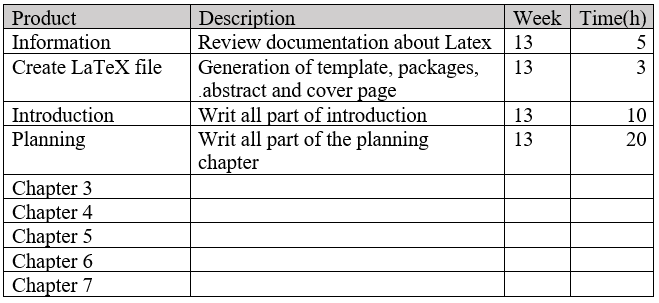
\includegraphics[width=0.9\textwidth]{imagenes/it5.png}\\[1.4cm]

\chapter{Theory Background}
\section{Introduction}
Cryptanalysis is the technique of extracting useful information about the key by observing the plaintext and cipher text using cryptanalysis try to break the secrecy provided by the cipher. There is no fixed method for cryptanalysis and every cipher is a different challenge to the attacker and hence demands different insight to attack\cite{jha2011cryptanalysis},The study of cipher text in an attempt to restore the message to plaintext is known as cryptanalysis. Cryptanalysis is equally mathematically challenging and complex as cryptography. Because of the complexity involved with cryptanalysis work this document is only focused on the basic techniques needed to decipher monoalphabetic encryption ciphers and cryptograms\cite{smith2001basic}.
In this chapter, explained the history of cryptanalysis, the technology of cryptanalysis, transposition cipher, substitution cipher and description genetics algorithm (GA).

\section{Cryptanalysis}
Cryptanalysis is the technique of deriving the original
message from the ciphertext without any prior knowledge of
secret key or derivation of key from the ciphertext. A general
technique for cryptanalysis, applicable to all cryptographic
algorithms is to try all the possible keys until the correct key
is matched, it is known as exhaustive key search. With every
passing day, the computing ability of hardware is increasing
manifold; therefore it becomes necessary to use long keys for
avoiding exhaustive key search \cite{bokhari2012cryptanalysis} and till today, many cryptanalytic attacks are developed based on these. Each variant of these have different methods to find distinguisher and
based on the distinguisher \cite{khurana2015variants}.

\begin{figure}[h]
	\centering
	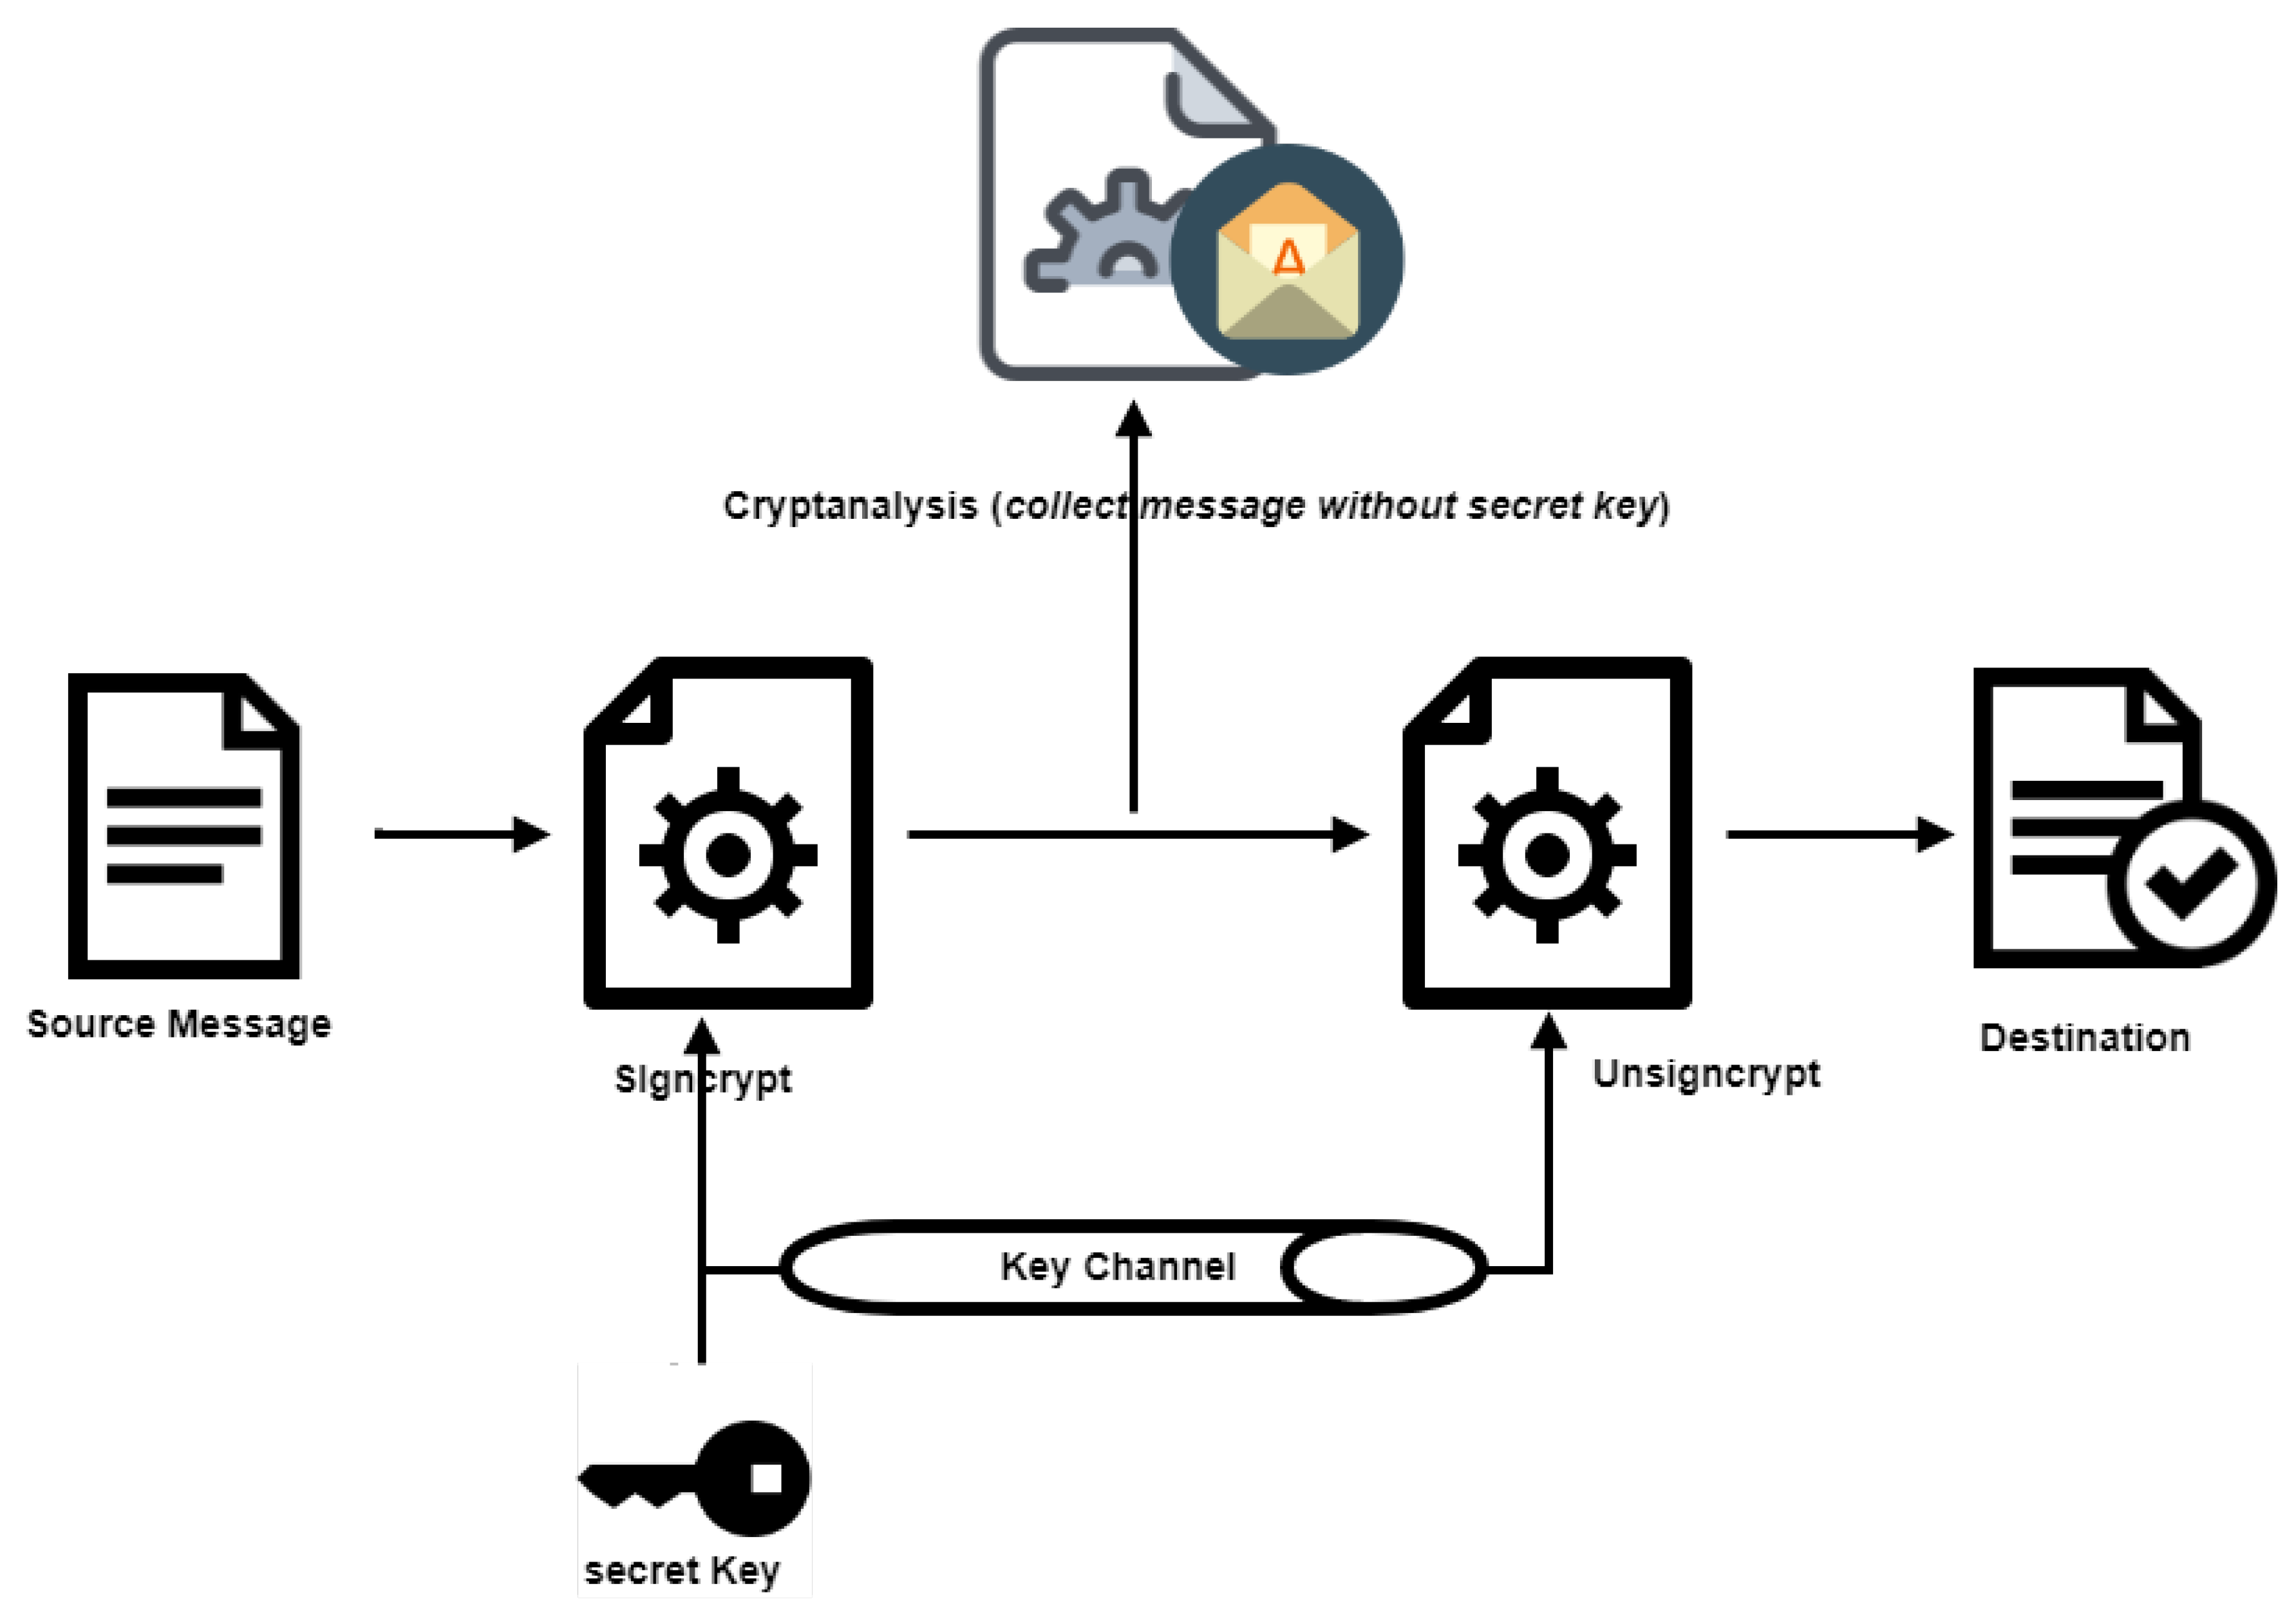
\includegraphics[scale=0.45]{imagenes/cryimage.png}
	\caption{Cryptanalysis cipher text}
\end{figure}

\subsection{CLASSIFICATION OF ATTACKS}

The main goal of a cryptanalyst is to obtain maximum
information about the plaintext (original data).Classification
of attacks can be done on following basis \cite{stallings2006cryptography}:
\begin{enumerate}
    \item{\textbf{Cipher text only attacks:} This is the most powerful attack. The
    attacker has only the knowledge of cipher text. This type of attack is
    successful only on the weakest of the ciphers.}
    \item{\textbf{Known plaintext attack:}attacker has the knowledge of plaintext and the corresponding cipher text, e.g. if an attacker is eavesdropping then  he can also guess the plaintext corresponding to some cipher texts depending upon the position or state of communication, in other words,  In this type a cryptanalyst have plaintext and their corresponding cipher text . Attacker tries to find out the relation between these two.}
    \item{\textbf{Chosen plaintext:}the attacker can choose its plaintext and get the cipher text corresponding to those chosen cipher text or The attacker obtain the various ciphertext corresponding to an arbitrary set of plaintext. }
    \item{\textbf{Chosen cipher text:} attacker is able to get the decrypted plaintext
    corresponding to his choice of cipher text. This attack is same as the
    chosen plaintext, but in a reverse direction which means The attacker obtain the various
    plaintext corresponding to an arbitrary set of cipher text}
    \item{\textbf{Adaptive chosen plaintext:}attacker first observes a large number of cipher texts. Based on the distribution of the cipher texts the attacker chooses a plaintext to get the corresponding cipher text which means the attacker chooses
    subsequent set of plaintext which is based on the information
    obtain from previous encryption methods.}
    \item{\textbf{Related Key: } This is a relatively new attack model. Here the attacker
    can encrypt two plaintext (same plaintext or the two plaintexts with a
    constant difference) with two keys, which have a fixed relation Between each other. This attack model is very weak as there is very little
    chance for the attacker to get encryption with two keys with a Constant
    relation. For lightweight block ciphers as the key is written to the device,
    this type of attack is not very probable.}
\end{enumerate}
\newpage
\subsection{Cryptanalytic technique}
In this section we will explain various cryptanalytic technique. As said earlier that, there are no fixed methods for cryptanalytic techniques for any block ciphers. But there are some methods which can be applied to every ciphers with some variation, though there can not be any guarantee that these methods may break the cipher. Cipher designers apply these methods to analyze security level for the computational security. Informally, broadly classify these techniques as brute force techniques non-brute force techniques. As the name suggest brute force techniques involves search of entire key space. Other techniques utilize the weakness in the structure of the ciphers to find key bits \cite{jha2011cryptanalysis}.

\subsubsection{Brute force technique:}
A brute-force attack is a can be used to attempt to decrypt any
encrypted data. Such an attack might be used when it is not possible to take
advantage of other weaknesses in an encryption system (if any exist) that
would make the task easier. When password guessing, this method is very
fast when used to check all short passwords, but for longer passwords other
methods such as the dictionary attack are used because a brute-force search
takes too long. Longer passwords, passphrases and keys have more
possible values, making them exponentially more difficult to crack than
shorter ones. can be made less effective by obfuscating the data to be
encoded making it more difficult for an attacker to recognize when the code
has been cracked or by making the attacker do more work to test each guess \cite{jha2011cryptanalysis}.

\subsubsection{Non-brute force techniques:}
In a non-brute-force attack, a single (usually common) password is
tested against multiple usernames or encrypted files. The process may be
repeated for a select few passwords. In such a strategy, the attacker is
Generally not targeting a specific user. Non brute-force attacks can be
mitigated by establishing a password policy that disallows common
passwords \cite{jha2011cryptanalysis}.
\newpage
\section{CipherText}
Ciphertext is encrypted text transformed from plaintext using an encryption algorithm. Ciphertext can't be read until it has been converted into  plaintext (decrypted) with a key. The decryption cipher is an algorithm that transforms the ciphertext back into plaintext.
The term cipher is sometimes used as a synonym for ciphertext. However, it refers to the method of encryption rather than the result.

\subsection{Types of ciphers}
There are various types of ciphers but We are focusing on only two of them that related to the work done , including:

\subsubsection{Transposition Cipher}
The transposition cipher is rearranged (change position only) the characters in the message but not change the characters. Transposition cipher have a pool of keys and ciphertext that rearranged the ciphertext for M times depended on the pool of keys. The output of transposition cipher saved in array of M locations we can called it \textit{plaintextArray}.
A simple transposition or permutation cipher works by breaking a message into fixed size blocks, and then permuting the characters within each block according to a fixed permutation, say P. The key to the transposition cipher is simply the permutation P. So, the transposition cipher has the property that the encrypted message contains all the characters that were in the plaintext message. In other words, the unigram statistics for the message are unchanged by the encryption process. The size of the permutation is known as the period. Let's consider an example of a transposition cipher with a period of ten 10, and a key P={7,10,4,2,8,1,5,9,6,3}. In this case, the message is broken into blocks of ten characters, and after encryption the seventh character in the block will be moved to position 1, the tenth moved character in the block will be moved to position 2, the forth is moved to position 3, the second to position 4, the eighth to position 5, the first to position 6, the fifth to the position 7, the ninth to the position 8, the sixth to the position 9 and the third to position 10.

In Table \ref{table:1} shows the key and the encryption process of the previously described transposition cipher. It can be noticed that the random string "X" was appended to the end of the message to enforce a message length, which is a multiple of the block size.It is also clear that thedecryption can be achieved by following the same process as encryption using the "inverse" of the encryption permutation. In this case the decryption key, P-1 is equal to {6,4,10,3,7,9,1,5, 8,2}.

\begin{table}[h!]
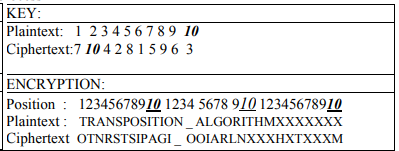
\includegraphics[width=0.9\textwidth]{imagenes/Transposition.png}\\
\caption{Transposition Cipher Example}
\label{table:1}
\end{table}
\newpage
\subsubsection{Substitution Cipher}
A cipher is an algorithm for encrypting plain text into cipher text and vice versa. The substitution cipher replaces every instance of a particular letter in the plain text with a different letter from the cipher text. Thus a substitution cipher key can be defined as the set of one-to-one mappings relating every letter in the plain text alphabet with the corresponding letter in cipher text alphabet. Such a key is normally defined using a table \ref{table:2}  and an example key is included below.
\begin{table}[h!]
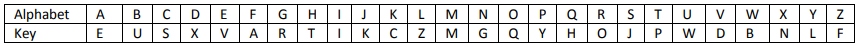
\includegraphics[width=0.9\textwidth]{imagenes/substitustion.png}\\
\caption{Substitution Cipher Example}
\label{table:2}
\end{table}

Thus the \textit{\textbf{HERE THE UNIVERSITY OF GRANADA}} can be encrypted to \textit{\textbf{QVOV PQV WGIDVOJPL QA ROEGEXE}},On the surface this cipher seems to be a strong one since there are 26 possibilities to choose from for the
first letter, 25 for the second, 24 for the third and so on. One can clearly see that there are in fact 26!
possible keys. 

\begin{equation} 26!= 26 * 25 * 24 * … * 1 = 4.03^{26} \end{equation}

However this cipher is particularly vulnerable to a technique known as frequency analysis since although it
does change the letters in the plain text to different ones in the cipher text it does not change the
underlying frequency of those letters.
Thus by comparing the frequencies of letters in the cipher text to a table of known letter frequencies for
the plain text language the key space can be reduced drastically. Furthermore you can also group letters
into n-grams where n represents the number of letters in the n-gram and look up the corresponding
frequencies for those \cite{brownbridge2007decrypting}. 
\newpage
\section{Genetic Algorithm}
Nature has always been a great source of inspiration to all mankind. Genetic Algorithms (GAs) are search based algorithms based on the concepts of natural selection and genetics. GAs are a subset of a much larger branch of computation known as Evolutionary Computation\cite{GAs}.
GAs were developed by John Holland and his students and colleagues at the University of Michigan, most notably David E. Goldberg and has since been tried on various optimization problems with a high degree of success\cite{GAs}.

The genetic algorithm is a general method of solving problems to
which no satisfactory, obvious, solution exists. It is based on the idea of
emulating the evolution of a species in nature, so the various components
of the Algorithm are roughly analogous to aspects of natural evolution.
Common mathematical tasks amenable to genetic solutions include
computing a curve to fit a set of data. Often these operators consist of
flipping a single.
Random bit of one individual or swapping two randomly selected
substrings from a pair of parents to generate a new child. To simulate
Darwinian survival of the fittest some representation of the fitness of the
individuals must be generated \cite{toemeh2007breaking}.

Genetic Algorithm Attack is more complicated than the  any other attack. This is because a pool of solutions is being maintained, rather than a single solution.
An extra level of complexity is also present because of the
need for a mating function and for a mutation function \cite{dimovski2003attacks}.

Genetic Algorithms are sufficiently randomized in nature, but they perform much better than random local search (in which we just try various random solutions, keeping track of the best so far), as they exploit historical information as well \cite{GAs}.
\newpage
\subsection{The steps of the genetic algorithm}
The genetic Algorithm has six steps which can evolve solutions to the search problem the following \cite{sastry2005genetic}:
\subsubsection{Initialization(Population)}
The initial population of candidate solutions is usually generated
randomly across the search space. However, domain-specific knowledge or other
information can be easily incorporated in the generation of the initial population.
The population is usually defined as a two dimensional array of size population, size x , chromosome size.
There are two primary methods to initialize a population in a GA. They are:
\subsubsection{Random Initialization:} Populate the initial population with completely random solutions.
\subsubsection{Heuristic initialization:} Populate the initial population using a known heuristic for the problem

\subsubsection{Evaluation(Fitness):}
Once the population is initialized, or an offspring population is created, the fitness values of the candidate solutions are evaluated.
A fitness function should possess the following characteristics:
\begin{enumerate}
    \item{The fitness function should be sufficiently fast to compute.}
    \item{It must quantitatively measure how fit a given solution is or how fit individuals can be produced from the given solution.}
\end{enumerate}

\subsubsection{Selection:} 
Selection allocates more copies to solutions with better fitness values and thus imposes the survival-of-the-fittest mechanism on the candidate solutions. The main idea of selection is to prefer better solutions to worse ones, and many selection procedures have been proposed to accomplish this idea, 
\subsubsection{Recombination(Crossover):}
Recombination combines bits and pieces of two or more parental solutions to create new, possibly better solutions (i.e. offspring). There are many ways of accomplishing this, and achieving competent performance depends on getting the recombination mechanism designed properly; but the primary idea to keep in mind is
that the offspring under recombination will not be identical to any particular parent and will instead combine parental traits in a novel manner \cite{goldberg1999using}.
\newpage
In GAs a crossover can be of following operators:
\subsubsection{Single Point Crossover:}
In this one-point crossover, a random crossover point is selected and the tails of its two parents are swapped to get new off-springs, as shown in figure \ref{onePointfigure}.

\begin{figure}[h]
	\centering
	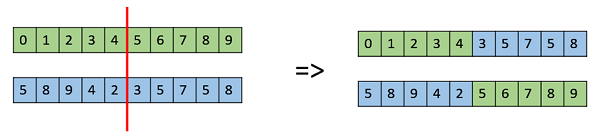
\includegraphics[scale=0.45]{imagenes/one_point_crossover.png}
    \caption{One Point Crossover operator}
    \label{onePointfigure}
\end{figure}

\subsubsection{Multi Point Crossover:}
Multi point crossover is a generalization of the one-point crossover wherein alternating segments are swapped to get new off-springs, as shown in figure \ref{MultiPointfigure}

\begin{figure}[h]
	\centering
	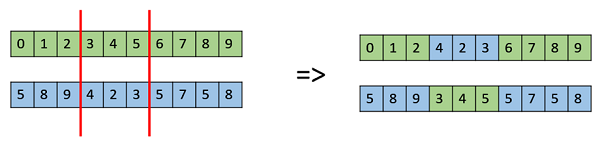
\includegraphics[scale=0.45]{imagenes/multi_point_crossover.png}
    \caption{Multi Point Crossover operator}
    \label{MultiPointfigure}
\end{figure}

\subsubsection{Uniform Crossover:}
In a uniform crossover, we don’t divide the chromosome into segments, rather we treat each gene separately. In this, we essentially flip a coin for each chromosome to decide whether or not it’ll be included in the off-spring. We can also bias the coin to one parent, to have more genetic material in the child from that parent, as shown in figure \ref{uniformfigure}.

\begin{figure}[h]
	\centering
	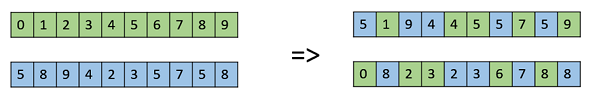
\includegraphics[scale=0.45]{imagenes/uniform_crossover.png}
    \caption{Uniform Crossover operator}
    \label{uniform}
\end{figure}

\subsubsection{Mutation:}
While recombination operates on two or more parental chromosomes,
mutation, locally but randomly, modifies a solution. Again, there are many variations of mutation, but it usually involves one or more changes that are made to
an individual’s trait or traits. In other words, mutation performs a random walk
in the vicinity of a candidate solution, as shown in figure \ref{mutation}.

\begin{figure}[h]
	\centering
	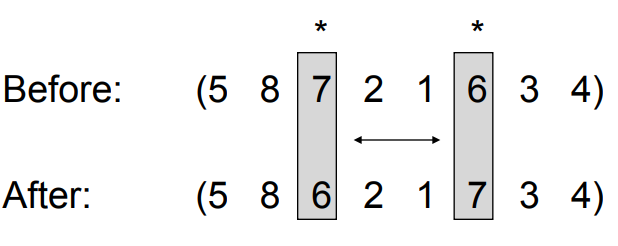
\includegraphics[scale=0.45]{imagenes/mutation.png}
    \caption{Mutation Example}
    \label{mutation}
\end{figure}

\subsubsection{Replacement:}
The offspring population created by selection,
recombination, and mutation replaces the original parental population.
Many replacement techniques such as elitist replacement, generationwise replacement and steady-state replacement methods are used in
GAs.

\subsection{Advantages and Limitations of Genetic Algorithms}
\subsubsection{Advantages}
GAs have various advantages which have made them immensely popular. These include:
\begin{enumerate}
    \item{Does not require any derivative information (which may not be available for many real-world problems).}
    \item{Is faster and more efficient as compared to the traditional methods.}
    \item{Has very good parallel capabilities.}
    \item{Optimizes both continuous and discrete functions and also multi-objective problems.}
    \item{Provides a list of “good” solutions and not just a single solution.}
    \item{Always gets an answer to the problem, which gets better over the time.}
    \item{Useful when the search space is very large and there are a large number of parameters involved.}
\end{enumerate}
\subsubsection{Limitations}
Like any technique, GAs also suffer from a few limitations. These include:
\begin{enumerate}
    \item{GAs are not suited for all problems, especially problems which are simple and for which derivative information is available.}
    \item{Fitness value is calculated repeatedly which might be computationally expensive for some problems.}
    \item{Being stochastic, there are no guarantees on the optimality or the quality of the solution.}
    \item{If not implemented properly, the GA may not converge to the optimal solution.}
\end{enumerate}

\subsection{Application areas of genetic algorithm (GA):}
Genetic Algorithms are primarily used in optimization problems of
various kinds, but they are frequently used in other application areas as
well. Some of the areas in which Genetic Algorithms are frequently used
explained in the following:
\subsubsection{Optimization:}
Genetic Algorithms are most commonly used in
optimization problems wherein we have to maximize or minimize.
Given objective function value under a given set of constraints. The
approach to solve Optimization problems has been highlighted
throughout the tutorial. 
\subsubsection{Economics:}
GAs are also used to characterize various economic
models like the cobweb model, game theory equilibrium resolution,
asset pricing, etc.
\subsubsection{Parallelization:}GAs also have very good parallel capabilities, and
prove to be very effective means in solving certain problems, and
provide a good area for research.
\subsubsection{Image Processing:} GAs are used for various digital image processing
(DIP) tasks as well like dense pixel matching.
\subsubsection{Vehicle routing problems:} With multiple soft time windows, multiple
depots and a heterogeneous fleet.
\subsubsection{Scheduling applications:}GAs are used to solve various scheduling
problems as well, particularly the time tabling problem.
\subsubsection{Machine Learning:}genetics based machine learning (GBML) is a
niche area in machine learning
\subsubsection{Robot Trajectory Generation:}GAs have been used to plan the path
which a robot arm takes by moving from one point to another.
\subsubsection{Parametric Design of Aircraft:}GAs have been used to design
aircrafts by varying the parameters and evolving better solutions.
\newpage


\chapter{Design and Implementation of Proposed Work}
This chapter will show the architectural, Algorithm, and class diagrams of the application,In this chapter also, the implementation of the proposed work will be explained which shows how genetic algorithm approach can be applied to cryptanalysis task, which does not have clear solution except for exhaustive search: breaking the Transposition and substitution cipher.
In this work, cryptanalysis used GA for searching the decryption key or getting maximum information about the decryption key. The Genetic Algorithm is a search and optimization techniques based On Darwin is the Principle of Natural Selection,
In Figure \ref{Cryptanalysis_flow} Flowchart of proposed method of cryptanalysis.
\begin{figure}[ht]
	\centering
	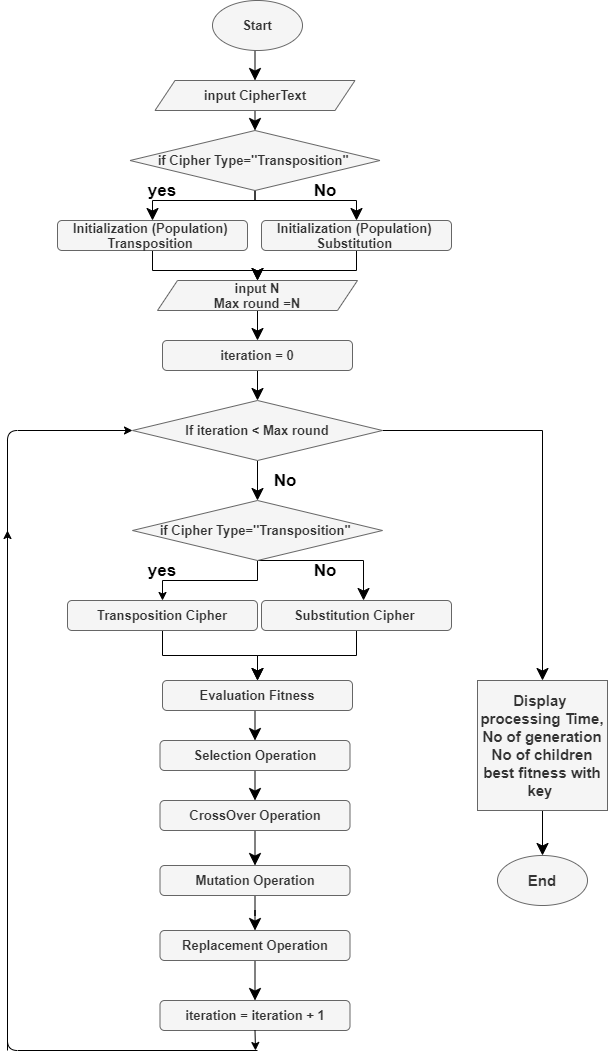
\includegraphics[width=.8\textwidth]{imagenes/FlowChartOfCry.png}
    \caption{Flowchart Of Proposed Method Of Cryptanalysis}
    \label{Cryptanalysis_flow}
\end{figure}
\section{Design of the work}
As we saw in Figure \ref{Cryptanalysis_flow} that we have nine main parts in the project Consequently, project design will content 9 dependency classes, first of them will be the main class which controls other classes as shown in Figure \ref{classes} and explains inheritance relationship between classes, In this section, we will explain the stages of project development as follows:
\newpage
\clearpage
\begin{figure}[h]
	\centering
	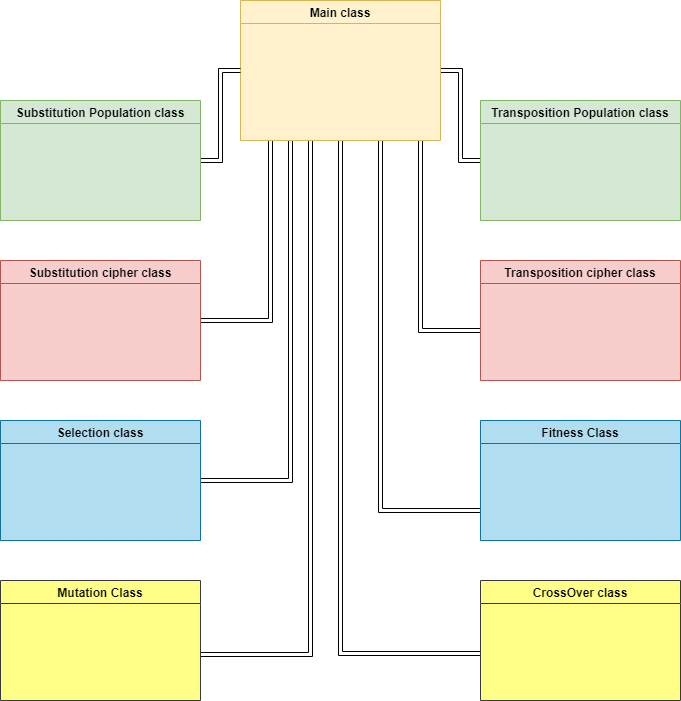
\includegraphics[width=.8\textwidth]{imagenes/classes.png}
    \caption{Inheritance relationship between the classes}
    \label{classes}
\end{figure}
\subsection{Population}
This part of the project is divided into two parts, depending on the cipher type:
\subsubsection{Transposition cipher population:}
In the initialization stage, generate a pool of random keys (size population), when the length of the key is N digits (chromosome size) and the pool size is M keys(size population). Also, The key condition is random and non-repetitive in each key. 
\subsubsection{Substitution  cipher population:}
on the other side, generate a pool of keys (size population), when the length of the key is 26 characters which equals the number of English letters (chromosome size) and the pool size is M keys(size population). Also, The key condition is random and non-repetitive in each key. These keys are changeable by the other stages of GA and the better one used in derivation the plaintext.
\subsection{Breaking Cipher}
in this stage, we will try to break the ciphertext using the keys which we got from the previous stage.
\subsubsection{Transposition Cipher:}
The transposition cipher is rearranged (change position only) the characters in the message but not change the characters. Transposition cipher has a pool of keys and ciphertext that rearranged the ciphertext for M times depending on the pool of keys. The output of transposition cipher saved in an array of M locations we can be called \textit{plaintext array}.
\subsubsection{Substitution Cipher:}
The substitution cipher replaces every instance of a particular letter in the ciphertext with a different letter from the cipher key, Thus a substitution cipher key can be defined as the set of one-to-one mappings relating every letter in the ciphertext alphabet with the corresponding letter in plaintext alphabet, so The Substitution cipher is changing the characters in the message but not change the characters positions, substitution cipher has a pool of keys and ciphertext that changed the ciphertext for M times depending on the pool of keys. The output of substitution cipher saved in an array of M locations which we can be called \textit{plaintext array}.
\subsection{Evaluation Fitness}
Fitness is evaluated based on the unigrams(one letter) frequencies, the bigrams (sequence of two letters) frequencies in the decrypted ciphertext, and Trigrams (sequence of three letters) frequencies in the decrypted ciphertext. the tables below illustrated the most popular bigrams and Trigrams in the English language. Trigrams and diagrams are computationally expensive the fitness calculation. The idea of the fitness function is the following \cite{Text_fitness}:
\begin{enumerate}
    \item{We take large text corpus and calculate the occurrences of unigrams, bigrams, and trigrams \begin{align*}& C^u_i, C^b_{ij}, C^t_{ijk} \end{align*}}
    \item{Then we sum all counters to get total sum of unigrams, bigrams and trigrams, \begin{align*}& S_u, S_b, S_t\end{align*}}
    \item{Then we calculate reference frequencies of each unigram, bigram and trigram,\begin{align*}& R^u_i = \frac{C^u_i}{S_u},R^b_{ij} = \frac{C^b_{ij}}{S_b},R^b_{ijk} =\frac{C^t_{ijk}}{S_t}\end{align*} }
    \item{Then, using the same method, we calculate the frequencies within the target text to obtain partial frequencies of each unigram, bigram and trigram, \begin{align*}& P^u_i, P^b_{ij}, P^t_{ijk} \end{align*} }.
    \item{Then we calculate the fitness score using the following formula:
    \begin{align*}
        F_i=\alpha \sum(R^u_i-P^u_i)+\beta \sum(R^b_{ij}-P^b_{ij})+\gamma \sum(R^t_{ijk}-P^t_{ijk})
    \end{align*}
where alpha, betha and gamma are the weights we assign to the importance of unigrams, bigrams and trigrams respectively. This implementation uses 1/6, 1/3 and 1/2, assigning most of the weight to trigrams}
\end{enumerate}
frequencies of unigrams, bigrams and trigrams are shown in the tables \ref{UI}\ref{TIBI1}\ref{TIBI2} respectively.
\begin{table}[h!]
    \centering
    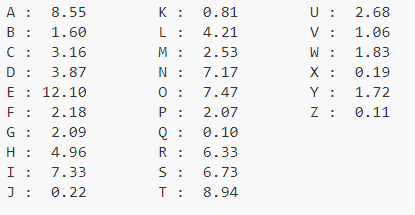
\includegraphics[width=0.8\textwidth]{imagenes/UI.png}\\
    \caption{English single letter frequencies}
    \label{UI}
\end{table}
\begin{table}[h!]
    \centering
    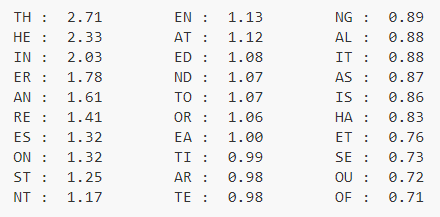
\includegraphics[width=0.8\textwidth]{imagenes/TIBI1.png}\\
    \caption{ The bigram frequencies}
    \label{TIBI1}
\end{table}
    \begin{table}[h!]
    \centering
    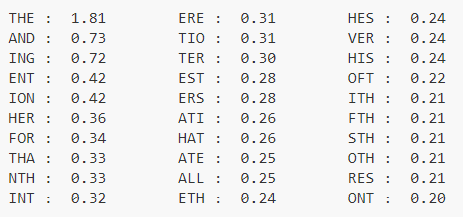
\includegraphics[width=0.8\textwidth]{imagenes/TIBI2.png}\\
    \caption{The trigram frequencies}
\label{TIBI2}
\end{table}
\newpage
\subsection{Selection}
In this operation, selection (choosing) the best keys only. The best key which has a high value of fitness. In the proposed work select only M/2 keys that have high fitness. To perform the selection operation needed a sorting function to sort pool of keys from high fitness to low fitness.

Fitness Proportionate Selection is one of the most popular ways of parent selection. In this stage, every individual can become a parent with a probability that is proportional to its fitness. Therefore, fitter individuals have a higher chance of mating and propagating their features to the next generation. Therefore, such a selection strategy applies a selection pressure to the more fit individuals in the population, evolving better individuals over time.
\subsection{CrossOver}
from the selection steps we got the best half of the population after calculating the fitness values, in this section, we generate a new population from the parents to get the children which represent the next generation, we can generate 2 children by using ( one point, two-point or uniform crossover operators )for each pair parents, but that gives us just half number of the original population, so can we use two methods to generate a new population, for instance, every 2 parents give us 4 children, the first 2 children are generated using one-point crossover operator and the other children are generated using uniform crossover operator,
in another way to keep the same number of population, we can keep the parents to the next generation, Through experiences, we can discuss which one is best to use, for that we applied all of them in this part to make the application more flexible.
\subsection{Mutation}
In this operation, applying the mutation operation for the new population. To perform the mutation operation, two random numbers generated such as R1, and R2 representing two positions in each key then swap between the value of the position R1 and the value of the position R2. Repeat this operation for all keys in the "new population" pool.
\subsection{Display The Results}
In this operation, display the plaintext (clear text is unencrypted information) for storage or transmission after decrypting the ciphertext. Also, display  the fitness values, the number of geneerations and te number individuals.
\section{Implementation of the proposed work}
\subsection{Population Steps}
the first class to start is Population.java in this class we created the Population which represents a set of chromosomes and each chromosome has the same length so, Population class has one constructor and many methods that follow:
\textsf{Population Constructor:} this constructor has two parameters:
\begin{itemize}
    \item{\textsf{NoOFkeys:} No. of chromosomes}
    \item{\textsf{lengthOFkey:} length of the chromosome.}
\end{itemize} 
under this Constructor, we can call all of the methods to create our population and show it. The first method is \textit{IFKEYEXIST} this method will generate a set of numbers between 1 and length of chromosome without repeat numbers (non-repetitive) and randomly, Method \textit{check} is created to ensure there are no duplicated numbers and check method has two parameters the first is an array of numbers are saved before and the second is a new number which will save in the same array,
and return true or false (if this new number exist in the array of the chromosome will return false in another case will return true and save it) after getting more then 2 chromosomes we have to check if there are duplicate chromosomes this step done with this method which called \textit{checkrow} which receive all of the chromosomes that saved before and new chromosome after that will compare between them to find if there are duplicated between these chromosomes, then will return false if there are no chromosomes duplicated and save it, if not, it will repeat the step of creating new chromosome.
\textsf{Note*}
this population will use to breaking Transposition cipher when we wanted to create a population to breaking Substitution Cipher we have created a new population class with some changes as follow:
the constructor of the substitution population class has just one parameter which is a no. of keys(No. of chromosomes) then we generated 26 characters from A to z randomly without repeating, so the length of the chromosome will be 26 characters are sorted randomly and non-repetitive.


\subsection{Trnsposition Steps}
The second step is Transposition Cipher, in this class Transposition.java we will try to get the origin text by using exchange the positions of characters as I explained in the section of Transposition Cipher, so if we have 16 keys, we can get 16 texts that may be the plaintext, in this class, we have 4 methods and one constructor, this class has:
\begin{itemize}
    \item{\textsf{Transposition constructor:} this Constructor has two parameters the array of keys which we got from Population class and ciphertext, then we will call methods that follow:}
\begin{enumerate}
    \item{\textsf{check if lenNotDivid} We created this method to enforce the message length, adding an "X" to the end of the message, making the message proportional to the key length.}
    \item{\textsf{change position} this method splits the ciphertext as blocks, the length of each block equals the length of the key, then call the SortbyKey method with sending one of the keys and one of the blocks to exchange the characters positions in each block.}
    \item{\textsf{SortByKey} this method receives one of the keys and one block of ciphertext and then exchanges the positions of all characters in that block depending on that key.}
    \item{\textsf{Print} this method called in the Transposition constructor to print the array of PlainText after doing the Transposition.}
\end{enumerate}
\end{itemize}


\subsection{Substitution Steps}
Substitution.java we will try to get the origin text by using change the  characters as I explained in the section of Substitution Cipher, so if we have 16 keys, we can get 16 texts that may be the plaintext, in this class, we created a constructor, under this constructor we created  new array to save texts after doing Substitution process, then we called a substitution method which responsible to change ciphertext to another text depending on the keys,
under this method, we convert each character in ciphertext to ASCII code then apply an equation to get the index of this character from the keys array,  \textit{an instance:}
\begin{tcolorbox}[breakable,notitle,boxrule=0pt,colback=blue!20,colframe=blue!20]
    {key= K H N E I B F G M D L U J V S P C Y Q R T X Z O  W  A\\
    ciphertex=HTSCRJ\\
    then we can get every character ASCII\\
    ASCII(H)=73\\
    ASCII(H)= ASCII(H)-65 so, ASCII(H)=8,\\
    GetIndex(8) form Key array\\
    H=G\\
    repeat this process to get every characters\\
    so, PlainText= GUOQTM
     }
    \end{tcolorbox}


\subsection{Fitness Evaluation steps}
with this step we created a new class, we called it, Fitness.java, this class contents on one constructor and set of methods to calculate fitness step by step, The first thing we did it is creating 6 arrays that follow:
\begin{itemize}
    \item{\textsf{monogram:} to save the unigram score(weight)}
    \item{\textsf{Twochar:}to save the bigram frequencies.}
    \item{\textsf{TwoCharVale} to save the bigram score(weight).}
    \item{\textsf{Threechar:}to save the trigram frequencies.}
    \item{\textsf{ThreeCharVale} to save the trigram score(weight).}
\end{itemize}
now, we are going to start with Fitness constructor which receives the Array of PlainTexts which we got  from Transipostion step and Array of keys(chromosomes), under this constructor, we initialized a set of arrays to save the summation of bigram frequencies of each PlainText, trigram frequencies summation, and unigram, and we created another array to save the final value of fitness for each PlainText, then we called methods to start calculating which follow:
\begin{itemize}
    \item{\textsf{FitnessMethod:} to save the unigram score(weight)}
    \item{\textsf{fitnessequation:}under this method, we will calculate the final value of fitness for each PlainText by using the equation and save it in Fitness array.}
\end{itemize}


\subsection{Selection Steps}
After getting fitness array for each PlainText from the previous step, it is time to select the best parents to generate a new population from those parents, let us firstly sort the fitness array descending then select the best half of that array by using high fitness, in the Selection.java class, we have one selection contracture which receives three parameters (the keys Array(chromosomes), PlainTexts Array, fitness Array ), under this contractor the first thing we have done it is initializing a set of arrays,
\begin{itemize}
    \item{\textsf{selectkey:} to save the best of keys.}
    \item{\textsf{selectPlinText:} to save the best plainText then we called two methods are the following:}
\end{itemize}
\begin{itemize}
    \item{\textsf{Sellsort:}this method sorts the fitness array at the same time sorts the keys and plaintexts arrays depending on the fitness values. note: the sell sort is one of the best sort ways are used to sort set of numbers \cite{goodrich2011randomized}.}
    \item{\textsf{Selection:} this method saves the best half of keys and plaintexts in other arrays and preppers them To produce a new generation.}
    \item{\textsf{Print:} to print the best keys and plaintexts.}
\end{itemize}
\subsection{CrossOver Steps}
in this class, we have to decide What better behavior to generate a new generation, for that, it's so important to step, as we explained in this section that there are many CrossOver operators to generate a new population dependent on the previous generation, we have used the 3 operators, before starting to create methods to perform these operators we had created a new class, we called it CrossOver class which contents one constructor to initialize set of arrays to save next generation and calls some methods that follow:
\begin{itemize}
    \item{\textsf{crossing:}  this method receives the set of best parents whose we got them from the Selection step, this method takes each parent individually and splits it into two equal parts then keeps the first part without change and do ascend sorts to the second then marriages them to represent a new child \textit{an example}
    \begin{tcolorbox}[breakable,notitle,boxrule=0pt,colback=blue!20,colframe=blue!20]
        {Parent 1 = 5 4 6 3 1 2 so, the Child 1= 5 4 6 1 2 3,\\
         Parent 2 = 1 6 5 4 3 2 so, the Child 2= 6 1 5 2 3 4}
        \end{tcolorbox}
    }
    \item{\textsf{onePoint:}this is another method to get a new population, but in this method, we will deal with two parents to generate Two children, as we explained in chapter two, so, this method takes two parents and keeps the first part of the first parent splits them into two equal parts for generating a first-child, keeps the first part of the first parent without change and copy the remaining unused numbers from the second parent to the first child, then it does the same process to generate a second-child, but it will keep the first part of the second parent without change and copy the remaining unused numbers from the first parent to the second child \textit{an example}.
    \begin{tcolorbox}[breakable,notitle,boxrule=0pt,colback=blue!20,colframe=blue!20]
        {Parent 1 = 5 4 6 |3 1 2\\ Parent 2 = 1 6 5 |4 3 2 \\
         so, child 1= 5 4 6| 1 3 2 and child 2= 1 6 5 | 4 3 2}
        \end{tcolorbox}
    }
    \item{\textsf{multiPoint:} this method is a generalization of the one-point crossover wherein alternating segments are swapped to get new off-springs \textit{an example}.
    \begin{tcolorbox}[breakable,notitle,boxrule=0pt,colback=blue!20,colframe=blue!20]
        { Parent 1 = 5 4 |6 3| 1 2\\ 
          Parent 2 = 1 6 |5 4| 3 2\\
        so, child 1 = 1 5 |3 6 |4 2 , and child 2= 6 3| 5 4 |1 2 }
        \end{tcolorbox}
    }
    \item{\textsf{marriagekeys:} The main purpose of creating this method is, as we know all of the CrossOver operators can generate N of children equals the number of parents Since the selection step gives us half of the original population Certainly the next generation will be half of the original population for that, this method receives two arrays the first array keeps all of the new children and the second array keeps (the best parent whose got it from the selection step) or apply another crossover operator to give us the second half of child, finally, it will marriage the arrays and keep them into newpopulionKey array which represents the next population.}
\end{itemize}
\subsection{Mutation Steps}
under this class Mutation.java we will mutate the gene, where We can determine a specific percentage of the generation then perform the mutation process on this part of the population only, so, the Mutation constructor receives the array of the new gene which we got from CrossOver steps with a mutation ratio in population, then we can mutate 2 positions for each child, these positions are random numbers in each child \textit{an example}.
\begin{tcolorbox}[breakable,notitle,boxrule=0pt,colback=blue!20,colframe=blue!20]
    {position 1 = 5 \\
     position 2 = 1 \\
     a chromosome = \textsf{1} 5 3 6 4 \textsf{2} \\
     so, chromosome = \textsf{2} 5 3 6 4 \textsf{1} }
    \end{tcolorbox}
Then we can call Print method to print the array of population after mutation process.
\chapter{Experimentation}
In this chapter, we will write all the issues related to the experimentation phase of the study, from the first decision-making to the last decision-making to validate the solutions. Throughout the following paragraphs, Arguments will be presented in defense of the decisions to be made and a sufficiently detailed description of the experiment will be presented so that the results can be easily interpreted.in this chapter we will get experimental results for each step of the application from population steps to mutation steps with giving the details of each step And make comparisons of the experimental results, These experiments are divided into two parts that depend on the cipher type.
so, we have two stages of the experimentation, which are:

\section{experimentation of Transposition Cipher}
In this part of the work, we will make experiments for the working steps performed to each step of GAs of Transposition cipher.
\subsection{experimentation of population step}
In this part of the work, we will make experiments for the working steps performed to each step of GAs of Transposition cipher.
in this section, we will make an experiment to generate a set of chromosomes(individuals) which represent the first population,  in this case, each chromosome has a set of numbers which represent DNA Which can not be repeated in another chromosome, for each problem, there is different chromosome type that we can define the chromosome (also sometimes called a genotype) is a set of parameters which define a proposed solution to the problem that the genetic algorithm is trying to solve. The set of all solutions is known as the population. The chromosome is often represented as a binary string, although a wide variety of other data structures are also used \cite{IVGeneticAlgorithm}.\\
\textsf{Experimental results 1 of Population step:}\\
    \colorbox{blue!30}{\textsf{     No. of chromosomes is: 12}}\\
    \colorbox{blue!30}{\textsf{     length of chromosome is: 6}}

\begin{table}[h!]
\centering
\begin{tabular}{l l}\hline
    Key(chromosome 0)&6 4 1 2 5 3\\ \hline 
    Key(chromosome 1)&3 5 1 2 4 6 \\ \hline 
    Key(chromosome 2)&1 5 2 4 6 3 \\ \hline 
    Key(chromosome 3)&1 4 3 2 6 5 \\ \hline 
    Key(chromosome 4)&3 5 2 4 1 6 \\ \hline 
    Key(chromosome 5)&4 3 5 1 6 2 \\ \hline 
    Key(chromosome 6)&6 4 3 2 5 1 \\ \hline 
    Key(chromosome 7)&3 1 5 4 6 2 \\ \hline 
    Key(chromosome 8)&3 6 2 5 4 1 \\ \hline 
    Key(chromosome 9)&5 3 2 4 1 6 \\ \hline 
    Key(chromosome 10)&4 1 5 3 2 6 \\ \hline 
    Key(chromosome 11)&1 3 6 4 2 5 \\ \hline  
\end{tabular}
\caption{Experimental results 1 Population step}

\end{table}



\textsf{Experimental results 1 of Population step:}\\
    \colorbox{blue!30}{\textsf{     No. of chromosomes is: 16}}\\

\begin{table}[H]
\centering
\begin{tabular}{l l}\hline
    Key(Chromosome0)&SEDJXKPIBCTRLVGZAOYQFHWUMN\\ \hline
    Key(Chromosome1)&VRQDBOFJXHYASCWLGKNMPZUITE\\ \hline
    Key(Chromosome2)&CMDABENOYRLKQGISPJTXVUWFZH\\ \hline
    Key(Chromosome3)&CJIBEVGYRTZWUMNSPFQOKHLDAX\\ \hline
    Key(Chromosome4)&ZDHTGNYBFMJRUKQVILXPWAECOS\\ \hline
    Key(Chromosome5)&VYDELMZQJTGSIRUNXAPFWKHOBC\\ \hline
    Key(Chromosome6)&RANHSXEPVUQDGTYBWKLZFJIOMC\\ \hline
    Key(Chromosome7)&DMPBJXAGOSWEVUTNYHRCFZLKQI\\ \hline
    Key(Chromosome8)&FZEBQTVDWXAIOGKMSHYNUPLCJR\\ \hline
    Key(Chromosome9)&CJYWORQPDMSNFEXGBTVIZLKUAH\\ \hline
    Key(Chromosome10)&GSCYDZXKNHTBMJEOPQLAIFWRUV\\ \hline
    Key(Chromosome11)&BNLVATPZRUSMCKHGXQDYIEJOWF\\ \hline
    Key(Chromosome12)&OWYFVAEZRJPHKGUDTMNCQIXSLB\\ \hline
    Key(Chromosome13)&NTDLUYPVISGXBFMOEKZAHWJRQC\\ \hline
    Key(Chromosome14)&FQRZKVHOCNEWGDPUMISLBTXYJA\\ \hline
    Key(Chromosome15)&XSUIQETDAYJRBPKMOCFLGVHNWZ\\ \hline
\end{tabular}
\caption{Experimental results 1 Population step}

\end{table}



\newpage
\subsection{experimentation of Transposition Cipher step}
in this section, we will try to break the ciphertext by using the decoding Transposition Algorithm to get the experimental results which will be:
\textsf{Experimental results 2 of Transposition Cipher step:}\\
    \colorbox{blue!30}{\textsf{     No. of chromosomes is: 20}}\\
    \colorbox{blue!30}{\textsf{     length of chromosome is: 10}}\\
    \colorbox{blue!30}{\textsf{     CipherText: siaTrtposnernioXphiC}}\\
    \colorbox{blue!30}{\textsf{     PlainText: TranspositionCipher}}
\begin{table}[h!]
\centering
\begin{tabular}{l l}\hline
    Plaintexts 0&aonTprtssinhCipoXier\\ \hline
    Plaintexts 1&snTtpaisroeCiXpnrioh\\ \hline
    Plaintexts 2&otrissnpaThXorieCpni\\ \hline
    Plaintexts 3&srnaptoiTsioCnpXhrie\\ \hline
    Plaintexts 4&apiotnsrTsnprhXCeoii\\ \hline
    Plaintexts 5&nosTrtispaCheioXripn\\ \hline
    Plaintexts 6&asTsnrtiponeiiCoXrph\\ \hline
    Plaintexts 7&itroasspnTrXohneipCi\\ \hline
    Plaintexts 8&ossipTrantheirpionCX\\ \hline
    Plaintexts 9&TaosnsriptinhiCeorpX\\ \hline
    Plaintexts 10&tnTposiarsXCiphirnoe\\ \hline
    Plaintexts 11&istnopsrTareXChpioin\\ \hline
    Plaintexts 12&poitsTanrsphrXiinCoe\\ \hline
    Plaintexts 13&iTaotrpsnsrinhXopeCi\\ \hline
    Plaintexts 14&TpotnasisriphXCnireo\\ \hline
    Plaintexts 15&nTstoripsaCieXhorpin\\ \hline
    Plaintexts 16&oastiprnsThniXrpoCei\\ \hline
    Plaintexts 17&rsostpnTaioiheXpCinr\\ \hline
    Plaintexts 18&riTsaopnstorienhpCiX\\ \hline
    Plaintexts 19&sspTtnraoieipiXConhr\\ \hline
\end{tabular}
\caption{Experimental results 2 Transposition Cipher}

\end{table}
\textsf{Experimental results 2 of Transposition Cipher step:}\\
    \colorbox{blue!30}{\textsf{     No. of chromosomes is: 20}}\\
    \colorbox{blue!30}{\textsf{     length of chromosome is: 10}}\\
    \colorbox{blue!30}{\textsf{     CipherText: siaTrtposnernioXphiC}}\\
    \colorbox{blue!30}{\textsf{     PlainText: TranspositionCipher}}
\begin{table}[h!]
\centering
\begin{tabular}{l l}\hline
    Plaintexts 0&aonTprtssinhCipoXier\\ \hline
    Plaintexts 1&snTtpaisroeCiXpnrioh\\ \hline
    Plaintexts 2&otrissnpaThXorieCpni\\ \hline
    Plaintexts 3&srnaptoiTsioCnpXhrie\\ \hline
    Plaintexts 4&apiotnsrTsnprhXCeoii\\ \hline
    Plaintexts 5&nosTrtispaCheioXripn\\ \hline
    Plaintexts 6&asTsnrtiponeiiCoXrph\\ \hline
    Plaintexts 7&itroasspnTrXohneipCi\\ \hline
    Plaintexts 8&ossipTrantheirpionCX\\ \hline
    Plaintexts 9&TaosnsriptinhiCeorpX\\ \hline
    Plaintexts 10&tnTposiarsXCiphirnoe\\ \hline
    Plaintexts 11&istnopsrTareXChpioin\\ \hline
    Plaintexts 12&poitsTanrsphrXiinCoe\\ \hline
    Plaintexts 13&iTaotrpsnsrinhXopeCi\\ \hline
    Plaintexts 14&TpotnasisriphXCnireo\\ \hline
    Plaintexts 15&nTstoripsaCieXhorpin\\ \hline
    Plaintexts 16&oastiprnsThniXrpoCei\\ \hline
    Plaintexts 17&rsostpnTaioiheXpCinr\\ \hline
    Plaintexts 18&riTsaopnstorienhpCiX\\ \hline
    Plaintexts 19&sspTtnraoieipiXConhr\\ \hline
\end{tabular}
\caption{Experimental results 2 Transposition Cipher}

\end{table}
\newpage
\subsection{experimentation of Fitness step}
now, we will get the preliminary experimental results to fitness step which will be:\\
\textsf{Experimental results 2 of Fitness step:}\\
    \colorbox{blue!30}{\textsf{     No. of chromosomes is: 20}}\\
    \colorbox{blue!30}{\textsf{     length of chromosome is: 10}}\\
    \colorbox{blue!30}{\textsf{     CipherText: siaTrtposnernioXphiC}}\\
    \colorbox{blue!30}{\textsf{     PlainText: TranspositionCipher}}

\begin{table}[H]
\centering
\begin{tabular}{l l}
    \hline
    \cellcolor[gray]{0.9} PlainTexs& \cellcolor[gray]{0.9} Fitness\\ \hline
    aonTprtssinhCipoXier&(15.4316648154)\\ \hline  
snTtpaisroeCiXpnrioh&(13.3783329054)\\ \hline  
otrissnpaThXorieCpni&(15.6483316654)\\ \hline  
srnaptoiTsioCnpXhrie&(13.3466662654)\\ \hline  
apiotnsrTsnprhXCeoii&(12.4366669154)\\ \hline  
nosTrtispaCheioXripn&(15.0066651054)\\ \hline  
asTsnrtiponeiiCoXrph&(14.4783321054)\\ \hline  
itroasspnTrXohneipCi&(13.799999275400001)\\ \hline  
ossipTrantheirpionCX&(17.2883305354)\\ \hline  
TaosnsriptinhiCeorpX&(14.4116655554)\\ \hline  
tnTposiarsXCiphirnoe&(13.4383328654)\\ \hline  
istnopsrTareXChpioin&(15.5483314054)\\ \hline  
poitsTanrsphrXiinCoe&(15.2149983254)\\ \hline  
iTaotrpsnsrinhXopeCi&(13.8866659454)\\ \hline  
TpotnasisriphXCnireo&(13.8783325354)\\ \hline  
nTstoripsaCieXhorpin&(15.5849980554)\\ \hline  
oastiprnsThniXrpoCei&(15.6816649754)\\ \hline  
rsostpnTaioiheXpCinr&(15.7466646554)\\ \hline  
riTsaopnstorienhpCiX&(14.943331785400002)\\ \hline  
sspTtnraoieipiXConhr&(13.0416664754)\\ \hline  
\end{tabular}
\caption{Experimental results 2 of Fitness step}

\end{table}



\textsf{Experimental results 2 of Fitness step:}\\
    \colorbox{blue!30}{\textsf{     No. of chromosomes is: 20}}\\
    \colorbox{blue!30}{\textsf{     length of chromosome is: 10}}\\
    \colorbox{blue!30}{\textsf{     CipherText: siaTrtposnernioXphiC}}\\
    \colorbox{blue!30}{\textsf{     PlainText: TranspositionCipher}}

\begin{table}[H]
\centering
\begin{tabular}{l l}
    \hline
    \cellcolor[gray]{0.9} PlainTexs& \cellcolor[gray]{0.9} Fitness\\ \hline
    aonTprtssinhCipoXier&(15.4316648154)\\ \hline  
snTtpaisroeCiXpnrioh&(13.3783329054)\\ \hline  
otrissnpaThXorieCpni&(15.6483316654)\\ \hline  
srnaptoiTsioCnpXhrie&(13.3466662654)\\ \hline  
apiotnsrTsnprhXCeoii&(12.4366669154)\\ \hline  
nosTrtispaCheioXripn&(15.0066651054)\\ \hline  
asTsnrtiponeiiCoXrph&(14.4783321054)\\ \hline  
itroasspnTrXohneipCi&(13.799999275400001)\\ \hline  
ossipTrantheirpionCX&(17.2883305354)\\ \hline  
TaosnsriptinhiCeorpX&(14.4116655554)\\ \hline  
tnTposiarsXCiphirnoe&(13.4383328654)\\ \hline  
istnopsrTareXChpioin&(15.5483314054)\\ \hline  
poitsTanrsphrXiinCoe&(15.2149983254)\\ \hline  
iTaotrpsnsrinhXopeCi&(13.8866659454)\\ \hline  
TpotnasisriphXCnireo&(13.8783325354)\\ \hline  
nTstoripsaCieXhorpin&(15.5849980554)\\ \hline  
oastiprnsThniXrpoCei&(15.6816649754)\\ \hline  
rsostpnTaioiheXpCinr&(15.7466646554)\\ \hline  
riTsaopnstorienhpCiX&(14.943331785400002)\\ \hline  
sspTtnraoieipiXConhr&(13.0416664754)\\ \hline  
\end{tabular}
\caption{Experimental results 2 of Fitness step}

\end{table}



\newpage
\subsection{experimentation of Selection step}
in experimentation of Selection steps, we will get the data are sorted depending on fitness values then we will select the best chromosomes:
\textsf{Experimental results 2 of Selection step:}\\
    \colorbox{blue!30}{\textsf{     No. of chromosomes is: 24}}\\
    \colorbox{blue!30}{\textsf{     CipherText: pnTsarotoiisepnhiCXXrXXX}}\\
    \colorbox{blue!30}{\textsf{     PlainText: TranspositionCipher}}
\begin{table}[H]
\centering
\begin{tabular}{{ m{7cm} m{5.5cm} m{1cm}}}\hline
    (best Key(chromosome)) &(Plain text ) &(Fitness value )\\ \hline
 TQXUIEJONBYSZKPHCRAWDVGLFM    &ANTWRWHPAKIRKNPLHONX&            11.874\\ \hline 
 MZBWGVILEQJAKSNRCHUOFPYXTD    &UEMOHORNUSGHSENXRLEB&            10.976\\ \hline 
 SLNGHABEDCOVQPMRXYWKFIUTJZ    &WDSKYKRMWPHYPDMTREDN&            10.943\\ \hline 
 RWHLNQMEUDVZSOGBYKXPFTJACI    &XURPKPBGXONKOUGABEUH&            10.283\\ \hline 
 UBRKAHQGOZPMNCTJWLFDSVIYEX    &FOUDLDJTFCALCOTYJGOR&            9.808\\ \hline 
 ELGKODWTBANXPCRHVZJUQYFSIM    &JBEUZUHRJCOZCBRSHTBG&            9.335\\ \hline 
 JARUCOYVHBDTXISEFGZLKQWMNP    &ZHJLGLESZICGIHSMEVHR&            9.021\\ \hline 
 ZMRQGOYLFBIJPEXDHVSWACKNTU    &SFZWVWDXSEGVEFXNDLFR&            8.763\\ \hline 
 NPAMLEXYHOQFVIZKBCWUSDTRGJ    &WHNUCUKZWILCIHZRKYHA&            8.524\\ \hline 
 YCJWOQERHKXMPFVLINDSTUGZAB    &DHYSNSLVDFONFHVZLRHJ&            8.213\\ \hline 
 FSYPXBTCJZGHOVNIAWEQLDUMRK    &EJFQWQINEVXWVJNMICJY&            7.634\\ \hline 
 GTSLQFDOCAXZKEHYIBVPMRWUNJ    &VCGPBPYHVEQBECHUYOCS&            7.560\\ \hline 
 
\end{tabular}
\caption{Experimental results 2 Selection Step}
\end{table}



\textsf{Experimental results 2 of Selection step:}\\
    \colorbox{blue!30}{\textsf{     No. of chromosomes is: 24}}\\
    \colorbox{blue!30}{\textsf{     CipherText: pnTsarotoiisepnhiCXXrXXX}}\\
    \colorbox{blue!30}{\textsf{     PlainText: TranspositionCipher}}
\begin{table}[H]
\centering
\begin{tabular}{{ m{7cm} m{5.5cm} m{1cm}}}\hline
    (best Key(chromosome)) &(Plain text ) &(Fitness value )\\ \hline
 TQXUIEJONBYSZKPHCRAWDVGLFM    &ANTWRWHPAKIRKNPLHONX&            11.874\\ \hline 
 MZBWGVILEQJAKSNRCHUOFPYXTD    &UEMOHORNUSGHSENXRLEB&            10.976\\ \hline 
 SLNGHABEDCOVQPMRXYWKFIUTJZ    &WDSKYKRMWPHYPDMTREDN&            10.943\\ \hline 
 RWHLNQMEUDVZSOGBYKXPFTJACI    &XURPKPBGXONKOUGABEUH&            10.283\\ \hline 
 UBRKAHQGOZPMNCTJWLFDSVIYEX    &FOUDLDJTFCALCOTYJGOR&            9.808\\ \hline 
 ELGKODWTBANXPCRHVZJUQYFSIM    &JBEUZUHRJCOZCBRSHTBG&            9.335\\ \hline 
 JARUCOYVHBDTXISEFGZLKQWMNP    &ZHJLGLESZICGIHSMEVHR&            9.021\\ \hline 
 ZMRQGOYLFBIJPEXDHVSWACKNTU    &SFZWVWDXSEGVEFXNDLFR&            8.763\\ \hline 
 NPAMLEXYHOQFVIZKBCWUSDTRGJ    &WHNUCUKZWILCIHZRKYHA&            8.524\\ \hline 
 YCJWOQERHKXMPFVLINDSTUGZAB    &DHYSNSLVDFONFHVZLRHJ&            8.213\\ \hline 
 FSYPXBTCJZGHOVNIAWEQLDUMRK    &EJFQWQINEVXWVJNMICJY&            7.634\\ \hline 
 GTSLQFDOCAXZKEHYIBVPMRWUNJ    &VCGPBPYHVEQBECHUYOCS&            7.560\\ \hline 
 
\end{tabular}
\caption{Experimental results 2 Selection Step}
\end{table}



\newpage
\subsection{experimentation of CrossOver step}
in this section, we will make a set of experiments to test every CrossOver operator, in the first part of the experiments will be applied, one crossover operator on the best parents to get half of the next population then mix those parents with their children to generate population completely, and in the second part of the experiments we will applied two Crossover operatores on the best parents  to generate population completely without keeping those parents to next generation, the experiments be:\\
\\\textsf{Experimental results 1 of CrossOver step:}\\
    \colorbox{blue!30}{\textsf{     No. of chromosomes is: 12}}\\
    \colorbox{blue!30}{\textsf{     length of chromosome is: 6}}\\
    \colorbox{blue!30}{\textsf{     CrossOver Operator: Two Point}}\\
    \colorbox{blue!30}{\textsf{     Keeps best parent to next Population: true}}

    \begin{table}[H]
        \centering
        \begin{tabular}{{ l l }}\hline
            Parent 1& 5  3  2  4  1  6 \\ \hline
            Parent 2&  6  4  1  2  5  3 \\ \hline
            Parent 3&  4  1  5  3  2  6 \\ \hline
          Parent 4&  1  3  6  4  2  5 \\ \hline
          Parent 5&  3  5  1  2  4  6 \\ \hline
          Parent 6&  4  3  5  1  6  2 \\ \hline
          Child 1&  6  1  2  4  5  3 \\ \hline
          Child 2&  5  3  1  2  4  6 \\ \hline
          Child 3&   1  6  5  3  4  2 \\ \hline
          Child 4&   1  5  6  4  3  2 \\ \hline
          Child 5&  4  3  1  2  5  6 \\ \hline
          Child 6&   3  2  5  1  4  6\\ \hline
\end{tabular}
\caption{Experimental results 1 CrossOver Step}
\end{table}



\\\textsf{Experimental results 1 of CrossOver step:}\\
    \colorbox{blue!30}{\textsf{     No. of chromosomes is: 12}}\\
    \colorbox{blue!30}{\textsf{     length of chromosome is: 6}}\\
    \colorbox{blue!30}{\textsf{     CrossOver Operator: Two Point}}\\
    \colorbox{blue!30}{\textsf{     Keeps best parent to next Population: true}}

    \begin{table}[H]
        \centering
        \begin{tabular}{{ l l }}\hline
            Parent 1& 5  3  2  4  1  6 \\ \hline
            Parent 2&  6  4  1  2  5  3 \\ \hline
            Parent 3&  4  1  5  3  2  6 \\ \hline
          Parent 4&  1  3  6  4  2  5 \\ \hline
          Parent 5&  3  5  1  2  4  6 \\ \hline
          Parent 6&  4  3  5  1  6  2 \\ \hline
          Child 1&  6  1  2  4  5  3 \\ \hline
          Child 2&  5  3  1  2  4  6 \\ \hline
          Child 3&   1  6  5  3  4  2 \\ \hline
          Child 4&   1  5  6  4  3  2 \\ \hline
          Child 5&  4  3  1  2  5  6 \\ \hline
          Child 6&   3  2  5  1  4  6\\ \hline
\end{tabular}
\caption{Experimental results 1 CrossOver Step}
\end{table}



\newpage
\subsection{experimentation of Mutation step}
At this stage, we will obtain the experimental results after the mutation process to obtain the final population that will continue to live to form other generations, the experimental results be:\\
\textsf{Experimental results 2 of Mutation step:}\\
    \colorbox{blue!30}{\textsf{     No. of chromosomes is: 20}}\\
    \colorbox{blue!30}{\textsf{     length of chromosome is: 10}}\\
    \colorbox{blue!30}{\textsf{     CrossOver Operator:One Point and Crossing}}\\
    \colorbox{blue!30}{\textsf{     Keeps best parent to next Population: false}}\\
    \colorbox{blue!30}{\textsf{     Two random Postions(2 bits of chromosome): 3 , 5}}\\
    \begin{table}[H]
        \centering
        \begin{tabular}{{ l l }}\hline
            \multicolumn{2}{c}{Final Population} \\ \hline
            chromosome 1 &2  4  7  6  8  10  9  1  5  3 \\ \hline
            chromosome 2 & 4  10  1  8  9  2  6  7  5  3 \\ \hline
            chromosome 3 & 9  5  7  10  2  6  4  3  8  1 \\ \hline
            chromosome 4 &  6  4  3  10  9  5  2  7  1  8 \\ \hline
            chromosome 5 &  3  7  6  2  10  1  9  8  5  4 \\ \hline
            chromosome 6 &2  1  8  9  10  3  7  6  4  5 \\ \hline
            chromosome 7 &  9  10  6  4  1  3  7  2  5  8 \\ \hline
          chromosome 8 &  10  3  9  6  7  1  4  5  2  8 \\ \hline
          chromosome 9 &  3  7  5  4  10  2  1  6  9  8 \\ \hline
          chromosome 10 &  4  2  1  3  5  7  10  6  9  8 \\ \hline
          chromosome 11 &  2  4  7  6  8  1  3  5  9  10 \\ \hline
          chromosome 12 &  4  10  1  8  9  2  3  5  6  7 \\ \hline
          chromosome 13 &  9  5  7  10  2  1  3  4  6  8 \\ \hline
          chromosome 14 &  6  4  3  10  9  1  2  5  7  8 \\ \hline
          chromosome 15 &   3  7  6  2  10  1  4  5  8  9 \\ \hline
          chromosome 16 &  2  1  8  9  10  3  4  5  6  7 \\ \hline
          chromosome 17 &  9  10  6  4  1  2  3  5  7  8 \\ \hline
          chromosome 18 &  10  3  9  6  7  1  2  4  5  8 \\ \hline
            chromosome 19 &  3  7  5  4  10  1  2  6  8  9 \\ \hline
            chromosome 20 & 4  2  1  3  5  6  7  8  9  10 \\ \hline
\end{tabular}
\caption{Experimental results 2 Mutation Step}
\end{table}



\textsf{Experimental results 2 of Mutation step:}\\
    \colorbox{blue!30}{\textsf{     No. of chromosomes is: 20}}\\
    \colorbox{blue!30}{\textsf{     length of chromosome is: 10}}\\
    \colorbox{blue!30}{\textsf{     CrossOver Operator:One Point and Crossing}}\\
    \colorbox{blue!30}{\textsf{     Keeps best parent to next Population: false}}\\
    \colorbox{blue!30}{\textsf{     Two random Postions(2 bits of chromosome): 3 , 5}}\\
    \begin{table}[H]
        \centering
        \begin{tabular}{{ l l }}\hline
            \multicolumn{2}{c}{Final Population} \\ \hline
            chromosome 1 &2  4  7  6  8  10  9  1  5  3 \\ \hline
            chromosome 2 & 4  10  1  8  9  2  6  7  5  3 \\ \hline
            chromosome 3 & 9  5  7  10  2  6  4  3  8  1 \\ \hline
            chromosome 4 &  6  4  3  10  9  5  2  7  1  8 \\ \hline
            chromosome 5 &  3  7  6  2  10  1  9  8  5  4 \\ \hline
            chromosome 6 &2  1  8  9  10  3  7  6  4  5 \\ \hline
            chromosome 7 &  9  10  6  4  1  3  7  2  5  8 \\ \hline
          chromosome 8 &  10  3  9  6  7  1  4  5  2  8 \\ \hline
          chromosome 9 &  3  7  5  4  10  2  1  6  9  8 \\ \hline
          chromosome 10 &  4  2  1  3  5  7  10  6  9  8 \\ \hline
          chromosome 11 &  2  4  7  6  8  1  3  5  9  10 \\ \hline
          chromosome 12 &  4  10  1  8  9  2  3  5  6  7 \\ \hline
          chromosome 13 &  9  5  7  10  2  1  3  4  6  8 \\ \hline
          chromosome 14 &  6  4  3  10  9  1  2  5  7  8 \\ \hline
          chromosome 15 &   3  7  6  2  10  1  4  5  8  9 \\ \hline
          chromosome 16 &  2  1  8  9  10  3  4  5  6  7 \\ \hline
          chromosome 17 &  9  10  6  4  1  2  3  5  7  8 \\ \hline
          chromosome 18 &  10  3  9  6  7  1  2  4  5  8 \\ \hline
            chromosome 19 &  3  7  5  4  10  1  2  6  8  9 \\ \hline
            chromosome 20 & 4  2  1  3  5  6  7  8  9  10 \\ \hline
\end{tabular}
\caption{Experimental results 2 Mutation Step}
\end{table}



\newpage


\section{experimentation of Substitution Cipher}
In this part of the work, we will make experiments for the working steps performed to each step of GAs of Substitution cipher.
\subsection{experimentation of population step}
As we said in the experimentation of population section of the Transposition Cipher that for each problem, there is different chromosome type then we used Integer chromosome Type, with substitution cipher problem the Integer chromosome Type will not work, so we have to use Character  chromosome Type, also in this problem the chromosome length will be constant which be 26 chars from A to Z are generated randomly and non-repetitive.
\textsf{Experimental results 1 of Population step:}\\
    \colorbox{blue!30}{\textsf{     No. of chromosomes is: 16}}\\

\begin{table}[H]
\centering
\begin{tabular}{l l}\hline
    Key(Chromosome0)&SEDJXKPIBCTRLVGZAOYQFHWUMN\\ \hline
    Key(Chromosome1)&VRQDBOFJXHYASCWLGKNMPZUITE\\ \hline
    Key(Chromosome2)&CMDABENOYRLKQGISPJTXVUWFZH\\ \hline
    Key(Chromosome3)&CJIBEVGYRTZWUMNSPFQOKHLDAX\\ \hline
    Key(Chromosome4)&ZDHTGNYBFMJRUKQVILXPWAECOS\\ \hline
    Key(Chromosome5)&VYDELMZQJTGSIRUNXAPFWKHOBC\\ \hline
    Key(Chromosome6)&RANHSXEPVUQDGTYBWKLZFJIOMC\\ \hline
    Key(Chromosome7)&DMPBJXAGOSWEVUTNYHRCFZLKQI\\ \hline
    Key(Chromosome8)&FZEBQTVDWXAIOGKMSHYNUPLCJR\\ \hline
    Key(Chromosome9)&CJYWORQPDMSNFEXGBTVIZLKUAH\\ \hline
    Key(Chromosome10)&GSCYDZXKNHTBMJEOPQLAIFWRUV\\ \hline
    Key(Chromosome11)&BNLVATPZRUSMCKHGXQDYIEJOWF\\ \hline
    Key(Chromosome12)&OWYFVAEZRJPHKGUDTMNCQIXSLB\\ \hline
    Key(Chromosome13)&NTDLUYPVISGXBFMOEKZAHWJRQC\\ \hline
    Key(Chromosome14)&FQRZKVHOCNEWGDPUMISLBTXYJA\\ \hline
    Key(Chromosome15)&XSUIQETDAYJRBPKMOCFLGVHNWZ\\ \hline
\end{tabular}
\caption{Experimental results 1 Population step}

\end{table}



\textsf{Experimental results 1 of Population step:}\\
    \colorbox{blue!30}{\textsf{     No. of chromosomes is: 16}}\\

\begin{table}[H]
\centering
\begin{tabular}{l l}\hline
    Key(Chromosome0)&SEDJXKPIBCTRLVGZAOYQFHWUMN\\ \hline
    Key(Chromosome1)&VRQDBOFJXHYASCWLGKNMPZUITE\\ \hline
    Key(Chromosome2)&CMDABENOYRLKQGISPJTXVUWFZH\\ \hline
    Key(Chromosome3)&CJIBEVGYRTZWUMNSPFQOKHLDAX\\ \hline
    Key(Chromosome4)&ZDHTGNYBFMJRUKQVILXPWAECOS\\ \hline
    Key(Chromosome5)&VYDELMZQJTGSIRUNXAPFWKHOBC\\ \hline
    Key(Chromosome6)&RANHSXEPVUQDGTYBWKLZFJIOMC\\ \hline
    Key(Chromosome7)&DMPBJXAGOSWEVUTNYHRCFZLKQI\\ \hline
    Key(Chromosome8)&FZEBQTVDWXAIOGKMSHYNUPLCJR\\ \hline
    Key(Chromosome9)&CJYWORQPDMSNFEXGBTVIZLKUAH\\ \hline
    Key(Chromosome10)&GSCYDZXKNHTBMJEOPQLAIFWRUV\\ \hline
    Key(Chromosome11)&BNLVATPZRUSMCKHGXQDYIEJOWF\\ \hline
    Key(Chromosome12)&OWYFVAEZRJPHKGUDTMNCQIXSLB\\ \hline
    Key(Chromosome13)&NTDLUYPVISGXBFMOEKZAHWJRQC\\ \hline
    Key(Chromosome14)&FQRZKVHOCNEWGDPUMISLBTXYJA\\ \hline
    Key(Chromosome15)&XSUIQETDAYJRBPKMOCFLGVHNWZ\\ \hline
\end{tabular}
\caption{Experimental results 1 Population step}

\end{table}



\newpage
\subsection{experimentation of Substitution Cipher step}
\textsf{Experimental results 2 of Transposition Cipher step:}\\
    \colorbox{blue!30}{\textsf{     No. of chromosomes is: 20}}\\
    \colorbox{blue!30}{\textsf{     length of chromosome is: 10}}\\
    \colorbox{blue!30}{\textsf{     CipherText: siaTrtposnernioXphiC}}\\
    \colorbox{blue!30}{\textsf{     PlainText: TranspositionCipher}}
\begin{table}[h!]
\centering
\begin{tabular}{l l}\hline
    Plaintexts 0&aonTprtssinhCipoXier\\ \hline
    Plaintexts 1&snTtpaisroeCiXpnrioh\\ \hline
    Plaintexts 2&otrissnpaThXorieCpni\\ \hline
    Plaintexts 3&srnaptoiTsioCnpXhrie\\ \hline
    Plaintexts 4&apiotnsrTsnprhXCeoii\\ \hline
    Plaintexts 5&nosTrtispaCheioXripn\\ \hline
    Plaintexts 6&asTsnrtiponeiiCoXrph\\ \hline
    Plaintexts 7&itroasspnTrXohneipCi\\ \hline
    Plaintexts 8&ossipTrantheirpionCX\\ \hline
    Plaintexts 9&TaosnsriptinhiCeorpX\\ \hline
    Plaintexts 10&tnTposiarsXCiphirnoe\\ \hline
    Plaintexts 11&istnopsrTareXChpioin\\ \hline
    Plaintexts 12&poitsTanrsphrXiinCoe\\ \hline
    Plaintexts 13&iTaotrpsnsrinhXopeCi\\ \hline
    Plaintexts 14&TpotnasisriphXCnireo\\ \hline
    Plaintexts 15&nTstoripsaCieXhorpin\\ \hline
    Plaintexts 16&oastiprnsThniXrpoCei\\ \hline
    Plaintexts 17&rsostpnTaioiheXpCinr\\ \hline
    Plaintexts 18&riTsaopnstorienhpCiX\\ \hline
    Plaintexts 19&sspTtnraoieipiXConhr\\ \hline
\end{tabular}
\caption{Experimental results 2 Transposition Cipher}

\end{table}
\textsf{Experimental results 2 of Transposition Cipher step:}\\
    \colorbox{blue!30}{\textsf{     No. of chromosomes is: 20}}\\
    \colorbox{blue!30}{\textsf{     length of chromosome is: 10}}\\
    \colorbox{blue!30}{\textsf{     CipherText: siaTrtposnernioXphiC}}\\
    \colorbox{blue!30}{\textsf{     PlainText: TranspositionCipher}}
\begin{table}[h!]
\centering
\begin{tabular}{l l}\hline
    Plaintexts 0&aonTprtssinhCipoXier\\ \hline
    Plaintexts 1&snTtpaisroeCiXpnrioh\\ \hline
    Plaintexts 2&otrissnpaThXorieCpni\\ \hline
    Plaintexts 3&srnaptoiTsioCnpXhrie\\ \hline
    Plaintexts 4&apiotnsrTsnprhXCeoii\\ \hline
    Plaintexts 5&nosTrtispaCheioXripn\\ \hline
    Plaintexts 6&asTsnrtiponeiiCoXrph\\ \hline
    Plaintexts 7&itroasspnTrXohneipCi\\ \hline
    Plaintexts 8&ossipTrantheirpionCX\\ \hline
    Plaintexts 9&TaosnsriptinhiCeorpX\\ \hline
    Plaintexts 10&tnTposiarsXCiphirnoe\\ \hline
    Plaintexts 11&istnopsrTareXChpioin\\ \hline
    Plaintexts 12&poitsTanrsphrXiinCoe\\ \hline
    Plaintexts 13&iTaotrpsnsrinhXopeCi\\ \hline
    Plaintexts 14&TpotnasisriphXCnireo\\ \hline
    Plaintexts 15&nTstoripsaCieXhorpin\\ \hline
    Plaintexts 16&oastiprnsThniXrpoCei\\ \hline
    Plaintexts 17&rsostpnTaioiheXpCinr\\ \hline
    Plaintexts 18&riTsaopnstorienhpCiX\\ \hline
    Plaintexts 19&sspTtnraoieipiXConhr\\ \hline
\end{tabular}
\caption{Experimental results 2 Transposition Cipher}

\end{table}
\newpage
\subsection{experimentation of Fitness step}
\textsf{Experimental results 2 of Fitness step:}\\
    \colorbox{blue!30}{\textsf{     No. of chromosomes is: 20}}\\
    \colorbox{blue!30}{\textsf{     length of chromosome is: 10}}\\
    \colorbox{blue!30}{\textsf{     CipherText: siaTrtposnernioXphiC}}\\
    \colorbox{blue!30}{\textsf{     PlainText: TranspositionCipher}}

\begin{table}[H]
\centering
\begin{tabular}{l l}
    \hline
    \cellcolor[gray]{0.9} PlainTexs& \cellcolor[gray]{0.9} Fitness\\ \hline
    aonTprtssinhCipoXier&(15.4316648154)\\ \hline  
snTtpaisroeCiXpnrioh&(13.3783329054)\\ \hline  
otrissnpaThXorieCpni&(15.6483316654)\\ \hline  
srnaptoiTsioCnpXhrie&(13.3466662654)\\ \hline  
apiotnsrTsnprhXCeoii&(12.4366669154)\\ \hline  
nosTrtispaCheioXripn&(15.0066651054)\\ \hline  
asTsnrtiponeiiCoXrph&(14.4783321054)\\ \hline  
itroasspnTrXohneipCi&(13.799999275400001)\\ \hline  
ossipTrantheirpionCX&(17.2883305354)\\ \hline  
TaosnsriptinhiCeorpX&(14.4116655554)\\ \hline  
tnTposiarsXCiphirnoe&(13.4383328654)\\ \hline  
istnopsrTareXChpioin&(15.5483314054)\\ \hline  
poitsTanrsphrXiinCoe&(15.2149983254)\\ \hline  
iTaotrpsnsrinhXopeCi&(13.8866659454)\\ \hline  
TpotnasisriphXCnireo&(13.8783325354)\\ \hline  
nTstoripsaCieXhorpin&(15.5849980554)\\ \hline  
oastiprnsThniXrpoCei&(15.6816649754)\\ \hline  
rsostpnTaioiheXpCinr&(15.7466646554)\\ \hline  
riTsaopnstorienhpCiX&(14.943331785400002)\\ \hline  
sspTtnraoieipiXConhr&(13.0416664754)\\ \hline  
\end{tabular}
\caption{Experimental results 2 of Fitness step}

\end{table}



\textsf{Experimental results 2 of Fitness step:}\\
    \colorbox{blue!30}{\textsf{     No. of chromosomes is: 20}}\\
    \colorbox{blue!30}{\textsf{     length of chromosome is: 10}}\\
    \colorbox{blue!30}{\textsf{     CipherText: siaTrtposnernioXphiC}}\\
    \colorbox{blue!30}{\textsf{     PlainText: TranspositionCipher}}

\begin{table}[H]
\centering
\begin{tabular}{l l}
    \hline
    \cellcolor[gray]{0.9} PlainTexs& \cellcolor[gray]{0.9} Fitness\\ \hline
    aonTprtssinhCipoXier&(15.4316648154)\\ \hline  
snTtpaisroeCiXpnrioh&(13.3783329054)\\ \hline  
otrissnpaThXorieCpni&(15.6483316654)\\ \hline  
srnaptoiTsioCnpXhrie&(13.3466662654)\\ \hline  
apiotnsrTsnprhXCeoii&(12.4366669154)\\ \hline  
nosTrtispaCheioXripn&(15.0066651054)\\ \hline  
asTsnrtiponeiiCoXrph&(14.4783321054)\\ \hline  
itroasspnTrXohneipCi&(13.799999275400001)\\ \hline  
ossipTrantheirpionCX&(17.2883305354)\\ \hline  
TaosnsriptinhiCeorpX&(14.4116655554)\\ \hline  
tnTposiarsXCiphirnoe&(13.4383328654)\\ \hline  
istnopsrTareXChpioin&(15.5483314054)\\ \hline  
poitsTanrsphrXiinCoe&(15.2149983254)\\ \hline  
iTaotrpsnsrinhXopeCi&(13.8866659454)\\ \hline  
TpotnasisriphXCnireo&(13.8783325354)\\ \hline  
nTstoripsaCieXhorpin&(15.5849980554)\\ \hline  
oastiprnsThniXrpoCei&(15.6816649754)\\ \hline  
rsostpnTaioiheXpCinr&(15.7466646554)\\ \hline  
riTsaopnstorienhpCiX&(14.943331785400002)\\ \hline  
sspTtnraoieipiXConhr&(13.0416664754)\\ \hline  
\end{tabular}
\caption{Experimental results 2 of Fitness step}

\end{table}



\newpage
\subsection{experimentation of Selection step}
\textsf{Experimental results 2 of Selection step:}\\
    \colorbox{blue!30}{\textsf{     No. of chromosomes is: 24}}\\
    \colorbox{blue!30}{\textsf{     CipherText: pnTsarotoiisepnhiCXXrXXX}}\\
    \colorbox{blue!30}{\textsf{     PlainText: TranspositionCipher}}
\begin{table}[H]
\centering
\begin{tabular}{{ m{7cm} m{5.5cm} m{1cm}}}\hline
    (best Key(chromosome)) &(Plain text ) &(Fitness value )\\ \hline
 TQXUIEJONBYSZKPHCRAWDVGLFM    &ANTWRWHPAKIRKNPLHONX&            11.874\\ \hline 
 MZBWGVILEQJAKSNRCHUOFPYXTD    &UEMOHORNUSGHSENXRLEB&            10.976\\ \hline 
 SLNGHABEDCOVQPMRXYWKFIUTJZ    &WDSKYKRMWPHYPDMTREDN&            10.943\\ \hline 
 RWHLNQMEUDVZSOGBYKXPFTJACI    &XURPKPBGXONKOUGABEUH&            10.283\\ \hline 
 UBRKAHQGOZPMNCTJWLFDSVIYEX    &FOUDLDJTFCALCOTYJGOR&            9.808\\ \hline 
 ELGKODWTBANXPCRHVZJUQYFSIM    &JBEUZUHRJCOZCBRSHTBG&            9.335\\ \hline 
 JARUCOYVHBDTXISEFGZLKQWMNP    &ZHJLGLESZICGIHSMEVHR&            9.021\\ \hline 
 ZMRQGOYLFBIJPEXDHVSWACKNTU    &SFZWVWDXSEGVEFXNDLFR&            8.763\\ \hline 
 NPAMLEXYHOQFVIZKBCWUSDTRGJ    &WHNUCUKZWILCIHZRKYHA&            8.524\\ \hline 
 YCJWOQERHKXMPFVLINDSTUGZAB    &DHYSNSLVDFONFHVZLRHJ&            8.213\\ \hline 
 FSYPXBTCJZGHOVNIAWEQLDUMRK    &EJFQWQINEVXWVJNMICJY&            7.634\\ \hline 
 GTSLQFDOCAXZKEHYIBVPMRWUNJ    &VCGPBPYHVEQBECHUYOCS&            7.560\\ \hline 
 
\end{tabular}
\caption{Experimental results 2 Selection Step}
\end{table}



\textsf{Experimental results 2 of Selection step:}\\
    \colorbox{blue!30}{\textsf{     No. of chromosomes is: 24}}\\
    \colorbox{blue!30}{\textsf{     CipherText: pnTsarotoiisepnhiCXXrXXX}}\\
    \colorbox{blue!30}{\textsf{     PlainText: TranspositionCipher}}
\begin{table}[H]
\centering
\begin{tabular}{{ m{7cm} m{5.5cm} m{1cm}}}\hline
    (best Key(chromosome)) &(Plain text ) &(Fitness value )\\ \hline
 TQXUIEJONBYSZKPHCRAWDVGLFM    &ANTWRWHPAKIRKNPLHONX&            11.874\\ \hline 
 MZBWGVILEQJAKSNRCHUOFPYXTD    &UEMOHORNUSGHSENXRLEB&            10.976\\ \hline 
 SLNGHABEDCOVQPMRXYWKFIUTJZ    &WDSKYKRMWPHYPDMTREDN&            10.943\\ \hline 
 RWHLNQMEUDVZSOGBYKXPFTJACI    &XURPKPBGXONKOUGABEUH&            10.283\\ \hline 
 UBRKAHQGOZPMNCTJWLFDSVIYEX    &FOUDLDJTFCALCOTYJGOR&            9.808\\ \hline 
 ELGKODWTBANXPCRHVZJUQYFSIM    &JBEUZUHRJCOZCBRSHTBG&            9.335\\ \hline 
 JARUCOYVHBDTXISEFGZLKQWMNP    &ZHJLGLESZICGIHSMEVHR&            9.021\\ \hline 
 ZMRQGOYLFBIJPEXDHVSWACKNTU    &SFZWVWDXSEGVEFXNDLFR&            8.763\\ \hline 
 NPAMLEXYHOQFVIZKBCWUSDTRGJ    &WHNUCUKZWILCIHZRKYHA&            8.524\\ \hline 
 YCJWOQERHKXMPFVLINDSTUGZAB    &DHYSNSLVDFONFHVZLRHJ&            8.213\\ \hline 
 FSYPXBTCJZGHOVNIAWEQLDUMRK    &EJFQWQINEVXWVJNMICJY&            7.634\\ \hline 
 GTSLQFDOCAXZKEHYIBVPMRWUNJ    &VCGPBPYHVEQBECHUYOCS&            7.560\\ \hline 
 
\end{tabular}
\caption{Experimental results 2 Selection Step}
\end{table}



\newpage
\subsection{experimentation of CrossOver step}
\\\textsf{Experimental results 1 of CrossOver step:}\\
    \colorbox{blue!30}{\textsf{     No. of chromosomes is: 12}}\\
    \colorbox{blue!30}{\textsf{     length of chromosome is: 6}}\\
    \colorbox{blue!30}{\textsf{     CrossOver Operator: Two Point}}\\
    \colorbox{blue!30}{\textsf{     Keeps best parent to next Population: true}}

    \begin{table}[H]
        \centering
        \begin{tabular}{{ l l }}\hline
            Parent 1& 5  3  2  4  1  6 \\ \hline
            Parent 2&  6  4  1  2  5  3 \\ \hline
            Parent 3&  4  1  5  3  2  6 \\ \hline
          Parent 4&  1  3  6  4  2  5 \\ \hline
          Parent 5&  3  5  1  2  4  6 \\ \hline
          Parent 6&  4  3  5  1  6  2 \\ \hline
          Child 1&  6  1  2  4  5  3 \\ \hline
          Child 2&  5  3  1  2  4  6 \\ \hline
          Child 3&   1  6  5  3  4  2 \\ \hline
          Child 4&   1  5  6  4  3  2 \\ \hline
          Child 5&  4  3  1  2  5  6 \\ \hline
          Child 6&   3  2  5  1  4  6\\ \hline
\end{tabular}
\caption{Experimental results 1 CrossOver Step}
\end{table}



\\\textsf{Experimental results 1 of CrossOver step:}\\
    \colorbox{blue!30}{\textsf{     No. of chromosomes is: 12}}\\
    \colorbox{blue!30}{\textsf{     length of chromosome is: 6}}\\
    \colorbox{blue!30}{\textsf{     CrossOver Operator: Two Point}}\\
    \colorbox{blue!30}{\textsf{     Keeps best parent to next Population: true}}

    \begin{table}[H]
        \centering
        \begin{tabular}{{ l l }}\hline
            Parent 1& 5  3  2  4  1  6 \\ \hline
            Parent 2&  6  4  1  2  5  3 \\ \hline
            Parent 3&  4  1  5  3  2  6 \\ \hline
          Parent 4&  1  3  6  4  2  5 \\ \hline
          Parent 5&  3  5  1  2  4  6 \\ \hline
          Parent 6&  4  3  5  1  6  2 \\ \hline
          Child 1&  6  1  2  4  5  3 \\ \hline
          Child 2&  5  3  1  2  4  6 \\ \hline
          Child 3&   1  6  5  3  4  2 \\ \hline
          Child 4&   1  5  6  4  3  2 \\ \hline
          Child 5&  4  3  1  2  5  6 \\ \hline
          Child 6&   3  2  5  1  4  6\\ \hline
\end{tabular}
\caption{Experimental results 1 CrossOver Step}
\end{table}



\newpage
\subsection{experimentation of Mutation step}
\textsf{Experimental results 2 of Mutation step:}\\
    \colorbox{blue!30}{\textsf{     No. of chromosomes is: 20}}\\
    \colorbox{blue!30}{\textsf{     length of chromosome is: 10}}\\
    \colorbox{blue!30}{\textsf{     CrossOver Operator:One Point and Crossing}}\\
    \colorbox{blue!30}{\textsf{     Keeps best parent to next Population: false}}\\
    \colorbox{blue!30}{\textsf{     Two random Postions(2 bits of chromosome): 3 , 5}}\\
    \begin{table}[H]
        \centering
        \begin{tabular}{{ l l }}\hline
            \multicolumn{2}{c}{Final Population} \\ \hline
            chromosome 1 &2  4  7  6  8  10  9  1  5  3 \\ \hline
            chromosome 2 & 4  10  1  8  9  2  6  7  5  3 \\ \hline
            chromosome 3 & 9  5  7  10  2  6  4  3  8  1 \\ \hline
            chromosome 4 &  6  4  3  10  9  5  2  7  1  8 \\ \hline
            chromosome 5 &  3  7  6  2  10  1  9  8  5  4 \\ \hline
            chromosome 6 &2  1  8  9  10  3  7  6  4  5 \\ \hline
            chromosome 7 &  9  10  6  4  1  3  7  2  5  8 \\ \hline
          chromosome 8 &  10  3  9  6  7  1  4  5  2  8 \\ \hline
          chromosome 9 &  3  7  5  4  10  2  1  6  9  8 \\ \hline
          chromosome 10 &  4  2  1  3  5  7  10  6  9  8 \\ \hline
          chromosome 11 &  2  4  7  6  8  1  3  5  9  10 \\ \hline
          chromosome 12 &  4  10  1  8  9  2  3  5  6  7 \\ \hline
          chromosome 13 &  9  5  7  10  2  1  3  4  6  8 \\ \hline
          chromosome 14 &  6  4  3  10  9  1  2  5  7  8 \\ \hline
          chromosome 15 &   3  7  6  2  10  1  4  5  8  9 \\ \hline
          chromosome 16 &  2  1  8  9  10  3  4  5  6  7 \\ \hline
          chromosome 17 &  9  10  6  4  1  2  3  5  7  8 \\ \hline
          chromosome 18 &  10  3  9  6  7  1  2  4  5  8 \\ \hline
            chromosome 19 &  3  7  5  4  10  1  2  6  8  9 \\ \hline
            chromosome 20 & 4  2  1  3  5  6  7  8  9  10 \\ \hline
\end{tabular}
\caption{Experimental results 2 Mutation Step}
\end{table}



\textsf{Experimental results 2 of Mutation step:}\\
    \colorbox{blue!30}{\textsf{     No. of chromosomes is: 20}}\\
    \colorbox{blue!30}{\textsf{     length of chromosome is: 10}}\\
    \colorbox{blue!30}{\textsf{     CrossOver Operator:One Point and Crossing}}\\
    \colorbox{blue!30}{\textsf{     Keeps best parent to next Population: false}}\\
    \colorbox{blue!30}{\textsf{     Two random Postions(2 bits of chromosome): 3 , 5}}\\
    \begin{table}[H]
        \centering
        \begin{tabular}{{ l l }}\hline
            \multicolumn{2}{c}{Final Population} \\ \hline
            chromosome 1 &2  4  7  6  8  10  9  1  5  3 \\ \hline
            chromosome 2 & 4  10  1  8  9  2  6  7  5  3 \\ \hline
            chromosome 3 & 9  5  7  10  2  6  4  3  8  1 \\ \hline
            chromosome 4 &  6  4  3  10  9  5  2  7  1  8 \\ \hline
            chromosome 5 &  3  7  6  2  10  1  9  8  5  4 \\ \hline
            chromosome 6 &2  1  8  9  10  3  7  6  4  5 \\ \hline
            chromosome 7 &  9  10  6  4  1  3  7  2  5  8 \\ \hline
          chromosome 8 &  10  3  9  6  7  1  4  5  2  8 \\ \hline
          chromosome 9 &  3  7  5  4  10  2  1  6  9  8 \\ \hline
          chromosome 10 &  4  2  1  3  5  7  10  6  9  8 \\ \hline
          chromosome 11 &  2  4  7  6  8  1  3  5  9  10 \\ \hline
          chromosome 12 &  4  10  1  8  9  2  3  5  6  7 \\ \hline
          chromosome 13 &  9  5  7  10  2  1  3  4  6  8 \\ \hline
          chromosome 14 &  6  4  3  10  9  1  2  5  7  8 \\ \hline
          chromosome 15 &   3  7  6  2  10  1  4  5  8  9 \\ \hline
          chromosome 16 &  2  1  8  9  10  3  4  5  6  7 \\ \hline
          chromosome 17 &  9  10  6  4  1  2  3  5  7  8 \\ \hline
          chromosome 18 &  10  3  9  6  7  1  2  4  5  8 \\ \hline
            chromosome 19 &  3  7  5  4  10  1  2  6  8  9 \\ \hline
            chromosome 20 & 4  2  1  3  5  6  7  8  9  10 \\ \hline
\end{tabular}
\caption{Experimental results 2 Mutation Step}
\end{table}



\newpage
%\input{capitulos/06_Resultados}
%\input{capitulos/07_Conclusiones}

%
%%\chapter{Conclusiones y Trabajos Futuros}
%
%
\nocite{*}
\bibliography{bibliografia/bibliografia}\addcontentsline{toc}{chapter}{Bibliografía}
\bibliographystyle{unsrt}
%
%\appendix
%\input{apendices/manual_usuario/manual_usuario}
%%\input{apendices/paper/paper}
%\input{glosario/entradas_glosario}
% \addcontentsline{toc}{chapter}{Glosario}
% \printglossary
\chapter*{}
\thispagestyle{empty}

\end{document}